\documentclass[11pt,a4paper,english,oneside, pdf]{article}
\usepackage[margin=2.5cm]{geometry}
\usepackage[utf8]{inputenc} %Permite introducir directamente acentos: á en lugar de \'a etc.
\usepackage{mathtools}
\usepackage{palatino}
\usepackage{graphicx}
\usepackage{hyperref}

\title{BACoN analysis}
\author{Carmen Romo Luque}

\graphicspath{{/Users/romoluque_c/LEGEND/BACON/Analysis_documentation/images/}}

\begin{document}
	\maketitle
	
	\section{Introduction}	 
	 The BACoN detector is designed to investigate the scintillation properties of liquid argon when doped with xenon. The setup consists of a 100-liter cylindrical cryostat filled with liquid argon, featuring a single upward-facing PMT mounted at the bottom and four rows of three equidistantly spaced SiPMs. Each SiPM row is separated by 10 cm from the next one. On top of the cylinder, an Americium source is placed, emitting gammas and alphas that interact with the liquid, producing scintillation light. The first row of SiPMs is positioned close to the decay source and serves as the trigger system when all of them detect at least one photoelectron. These three SiPMs are collimated to prevent potential saturation effects.
	 
	 	\begin{figure}[!h]
	 	\begin{center}
	 		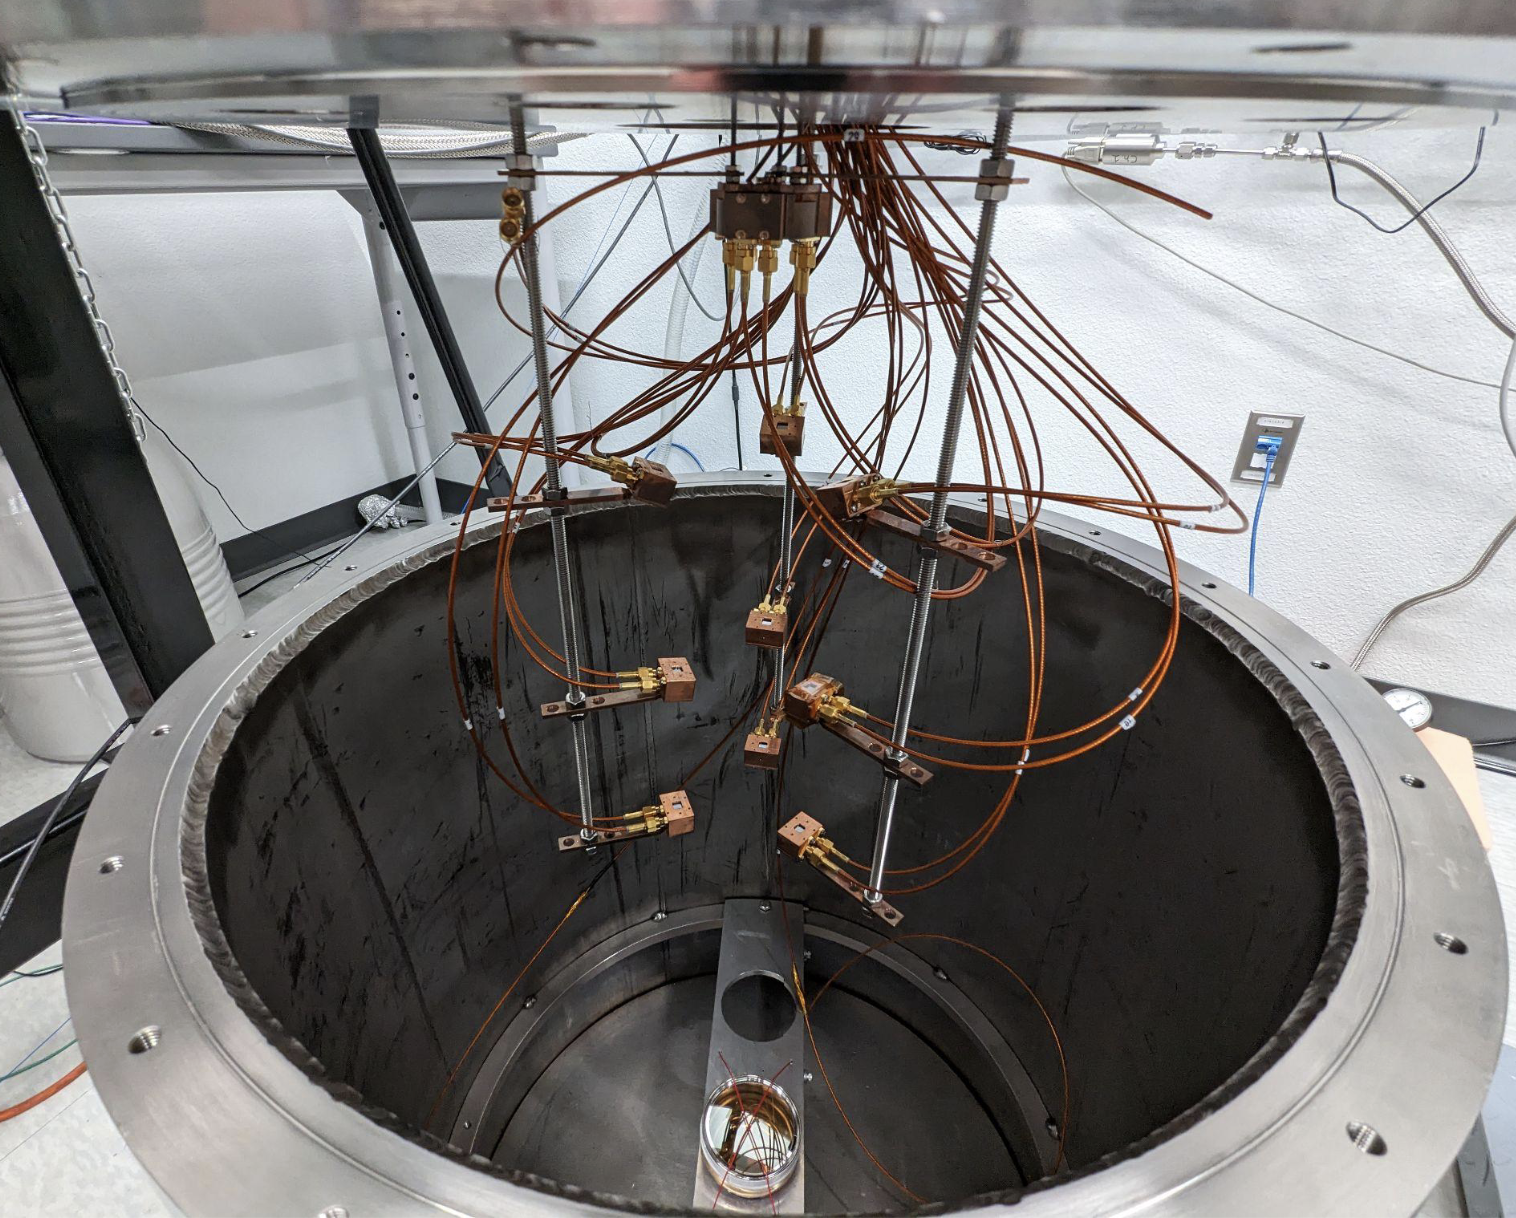
\includegraphics[width=9cm]{BACoN_picture_run2}
	 		\caption{New setup of the BACoN detector. The PMT is placed at the bottom of the chamber and 4 rows of SiPMs arranged around 10 cm apart, facing the americium source.}
	 		\label{fig:BACoN_picture_run2}
	 	\end{center}
	 \end{figure}
	 
	 The cryostat's liquid argon level is continuously monitored by measuring its weight. Additionally, the argon undergoes purification via a SAES PS4-MT3/15-R getter, which removes impurities such as H$_2$0, CO, CO$_2$, N$_2$, H$_2$, CH$_4$, reducing their concentrations to less than 1 part per billion (PPB) prior to liquefaction.
	
	\section{SiPM calibration in a dark box}
	\label{cal_dark_box}
	
	Maintaining the optimal performance of sensors in the BACoN system is crucial for accurate data collection, enabling the detection of variations in light levels within the detector. For this, periodic calibrations of the SiPMs are conducted to verify their proper functioning and stability. Despite employing the same sensor model across all SiPMs, variations in analog-to-digital conversion (ADC) counts in response to identical light inputs are inevitable. Hence, regular calibration of the SiPMs at the single photon level is imperative to standardize their responses and assess their long-term stability.
	
	Prior to installation within the chamber, the SiPMs were calibrated in a controlled environment using a dark box illuminated by a pulsed LED. The amplitude of the LED pulse utilized during calibration runs depended on various factors including the LED characteristics, the electronics chain, and the sensor gain. The light intensity was adjusted using an oscilloscope to achieve a few ADCs, guaranteeing operation at the single photoelectron level. Subsequently, pulse height spectra were generated by extracting the pulse heights. Given the low amplitude of pulses at the photoelectron level, they occasionally merge with dark counts, rendering them indistinguishable. Figure \ref{fig:wf_dark_box} presents an illustrative example of a waveform captured during a calibration run.
	
	\begin{figure}[!h]
		\begin{center}
			\includegraphics[width=12cm]{wf_dark_box_palatino.pdf}
			\caption{Example of a signal waveform of a SiPM tested in the dark box.}
			\label{fig:wf_dark_box}
		\end{center}
	\end{figure}

	
	First, we subtract the baseline of the waveform, which allows us to obtain the absolute height of the peaks. The baseline subtraction procedure can be performed by computing either the mean value or the mode of the entire waveform or just a certain range. Figure \ref{fig:wf_and_swf_dark_box_palatino} shows an example of a waveform before and after subtracting the baseline.
	
	\begin{figure}[!h]
		\begin{center}
			\includegraphics[width=11cm]{wf_and_swf_dark_box_palatino.pdf}
			\caption{Previous signal waveform and the waveform after subtracting its baseline.}
			\label{fig:wf_and_swf_dark_box_palatino}
		\end{center}
	\end{figure}
	
	Then, we compute the single photon spectra by getting the height of the peaks at the trigger region. Figure \ref{fig:summed_subtr_wf_trigger_region_col} shows the sum of all waveforms for one channel with the peak in the trigger region colored in grey.
	
	\begin{figure}[!h]
		\begin{center}
			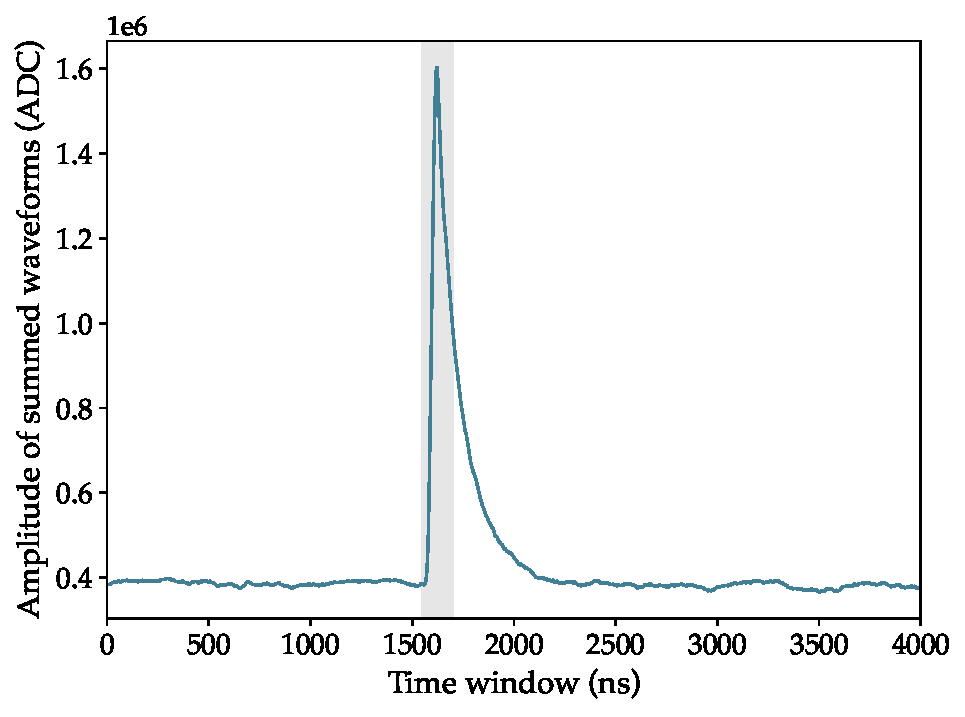
\includegraphics[width=11.5cm]{summed_subtr_wf_trigger_region_colored_palatino.pdf}
			\caption{Sum of all subtracted waveforms for one file for a chosen channel. The shadowed range corresponds to the trigger region.}
			\label{fig:summed_subtr_wf_trigger_region_col}
		\end{center}
	\end{figure}
	
	Subsequently, a histogram is generated displaying the heights of the peaks in the trigger window, allowing for the identification of individual single photoelectron peaks (refer to Figure \ref{fig:spectrum_black_box_fitted}). First, a poisson distribution of a certain number of gaussians is perfomed in order to extract the mean position of each photoelectron peak. The gain is then calculated from the spectrum using the distance between the pedestal peak and those for 1, 2, ...  photoelectrons.
	
	
	
	Then, the linear regression of the mean achieved enables the extraction of the conversion factor between ADC and photoelectrons. With these values, the response across all channels can be standardize.
	
	\begin{figure}[!h]
		\begin{center}
			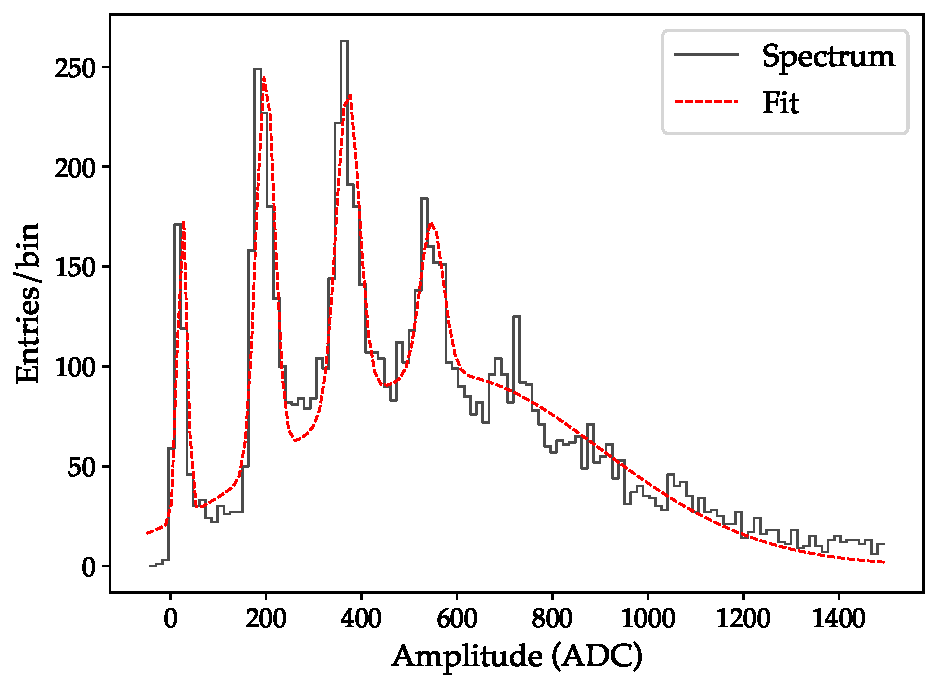
\includegraphics[width=11cm]{spectrum_black_box_fitted_palatino.pdf}
			\caption{Single pe spectrum for one channel showing the individual peaks. The distribution has been fitted of multiple Gaussian distributions, collectively following a Poisson distribution.}
			\label{fig:spectrum_black_box_fitted}
		\end{center}
	\end{figure}
	
	Figure \ref{fig:Gain_all_channels_black_box} shows the gain resulting from the 12 channels tested in the black box at two different bias voltages.

	\begin{figure}[!h]
		\begin{center}
			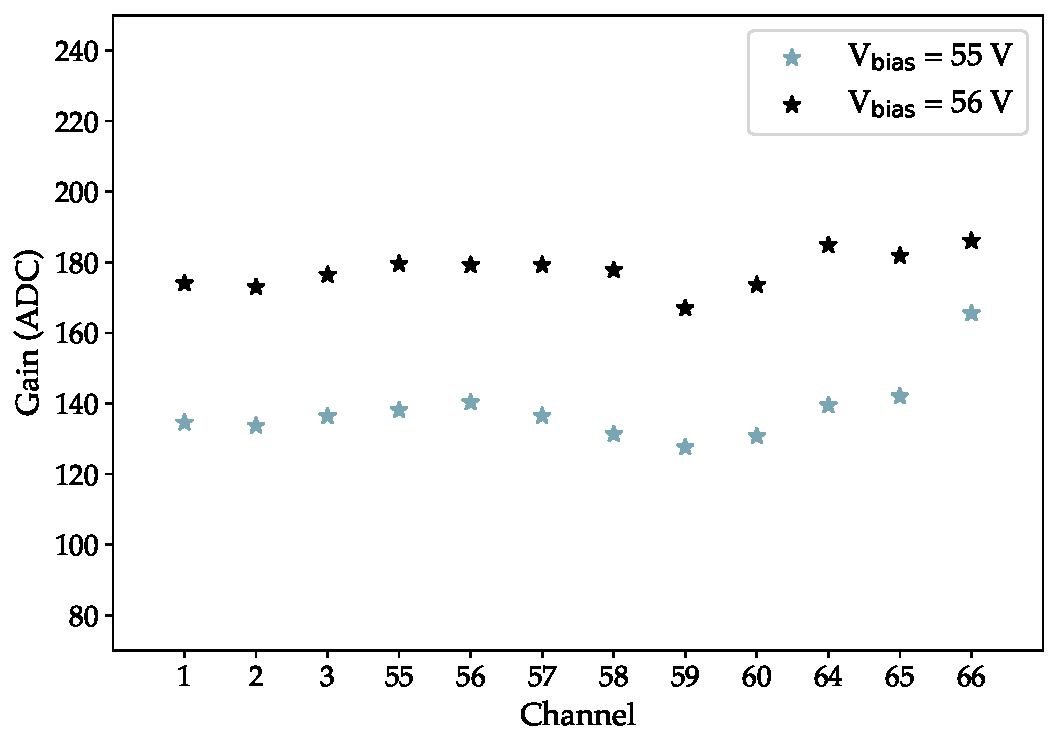
\includegraphics[width=11cm]{Gain_all_channels_black_box_palatino.pdf}
			\caption{Gain obtained for each channel at 55 V (blue) and 56 V (black) bias voltages.}
			\label{fig:Gain_all_channels_black_box}
		\end{center}
	\end{figure}
	
	%The data are processed by calculating the baseline and subtracting it for every event and sensor, and taking 2 $\mu$s integrals at the trigger time, giving rise to the spectra. The 2 $\mu$s integral width was chosen in NEXT for the standard calibration as a compromise between capturing all the light and the limitations imposed by the high level of noise in some channels \cite{internal_sipmCal_Andrew}.

	%The gain is then calculated from the spectrum using the distance between the pedestal peak and those for 1, 2, ...  photoelectrons. Figure \ref{fig:gain_spectrum_fits}-\textit{left} exhibits a fitted spectrum from a SensL SiPM of the NEXT-White detector with individual gaussian fits for every peak to show the linear relation between them, from which the gain is extracted (Figure \ref{fig:gain_spectrum_fits}-\textit{right}). The calibration results in average pedestals for each channel as well as the single photon conversion values \cite{internal_sipmCal_Andrew}.
	
	\section{SiPM calibration in the chamber}
	
	Ideally, a chamber should be equipped with LEDs for performing regular calibrations during data collection. That would allow us to monitor gain variations over time at a controlled light intensity, particularly important for long-term data acquisitions lasting several months or few years. Additionally, since we operate at low temperatures, the gains of the SiPMs won't match those obtained during black box calibration. However, in the absence of LEDs, we can still utilize low-light data for similar calibrations, though it's important to note that the values may differ.
	
	Due to the low temperature required to maintain argon in its liquid state within the BACoN detector, the bias voltage of the SiPMs needs to be reduced. This compensates for the decrease in breakdown voltage of the silicon diodes within the SiPM structure under reduced thermal conditions. At lower temperatures, the breakdown voltage tends to increase, meaning that the same bias voltage applied at room temperature could potentially cause the SiPMs to operate in a regime where the breakdown voltage is exceeded. This can lead to excess dark count rate and decreased performance. Therefore, reducing the bias voltage when operating SiPMs at lower temperatures helps ensure that they remain within their optimal operating conditions and maintain stable performance. That's the reason why the gains of the SiPMs inside the chamber are higher even at a lower bias voltage, as can be seen in Figure \ref{fig:gains_dark_box_and_BACoN}.
	
	\begin{figure}[!h]
		\begin{center}
			\includegraphics[width=11cm]{gains_dark_box_and_BACoN.pdf}
			\caption{Gain obtained for each normal channel at 55 V (blue) and 56 V (black) bias voltages in the dark box and at 46.7 V inside the BACoN detector.}
			\label{fig:gains_dark_box_and_BACoN}
		\end{center}
	\end{figure}
	
	
	\section{Data Run 2 analysis}
	
	The second period of data collection in BACoN began in mid-November 2023. Figure \ref{fig:event_example_all_SiPMs} shows the waveform for each channel for a particular event. Once the three trigger SiPMs detect one photon each, the event starts, and the rest of the channels (from channel 0 to 8) trigger as well. During the initial days, only argon was inside the chamber, and the gain of the trigger SiPMs was adjusted twice after several days (first on November 21st and then on December 2nd, as shown in Figure \ref{fig:Gain_trigger_channels_BACoN_run2}). The PMT malfunctioned and stopped working, so the data for these runs do not include that information. Additionally, in December 2023, channel 5 of the normal SiPMs started to have issues and was disconnected.
	
	\begin{figure}[!h]
		\begin{center}
			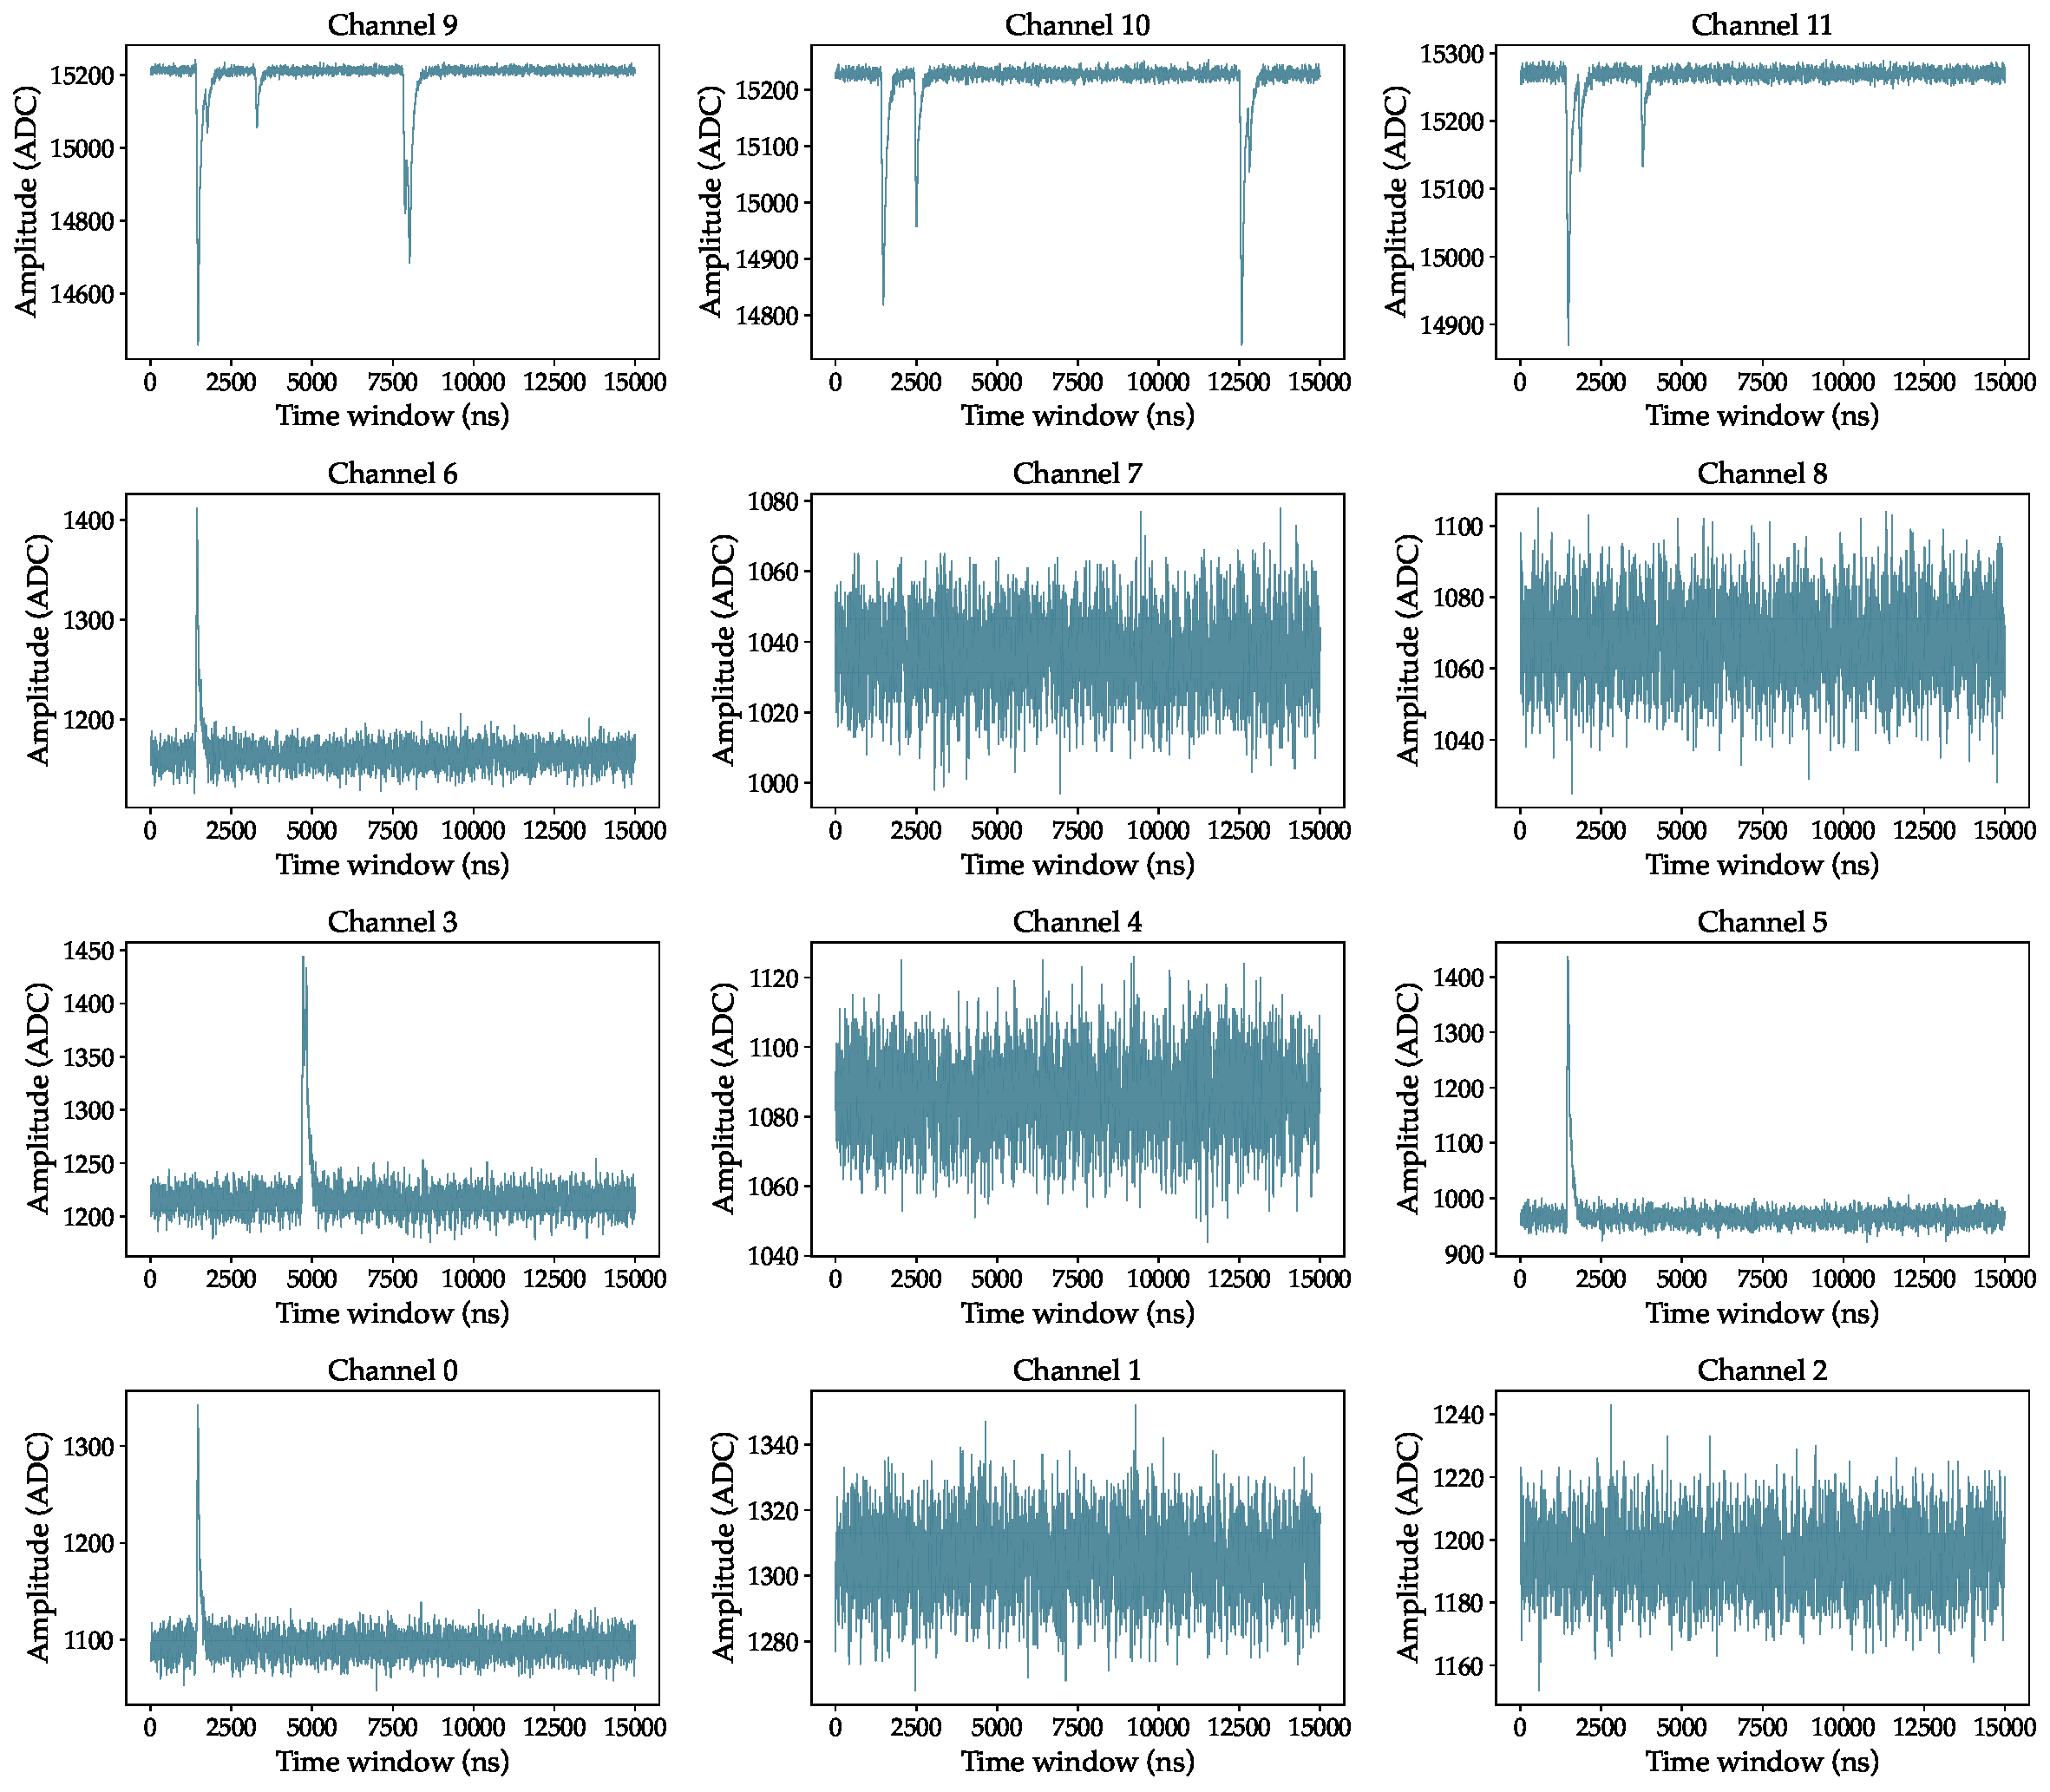
\includegraphics[width=16cm]{event_example_all_SiPMs.pdf}
			\caption{Raw waveforms of all channels for one particular event. Channels are sorted in closer proximity to the source, with channels 9, 10, and 11 being the closest to the source (in fact, they are the trigger SiPMs), while channels 0, 1, and 2 are the farthest from the source, closer to the bottom of the vessel.}
			\label{fig:event_example_all_SiPMs}
		\end{center}
	\end{figure}
	
	Figure \ref{fig:event_example_all_SiPMs} depicts the appearance of the data. In this specific event, besides the signal in the trigger SiPMs, which is required to store the event, other channels detect light, evident in the form of single peaks. Conversely, there are channels where no light is detected, and only the baseline originating from the electronics is visible in the waveform. In our setup, the signal from the trigger SiPMs is inverted due to the specific electronic chain for those channels. Therefore, an additional step in the analysis chain will be required to flip their signal.
	
	
	\begin{figure}[!h]
		\begin{center}
			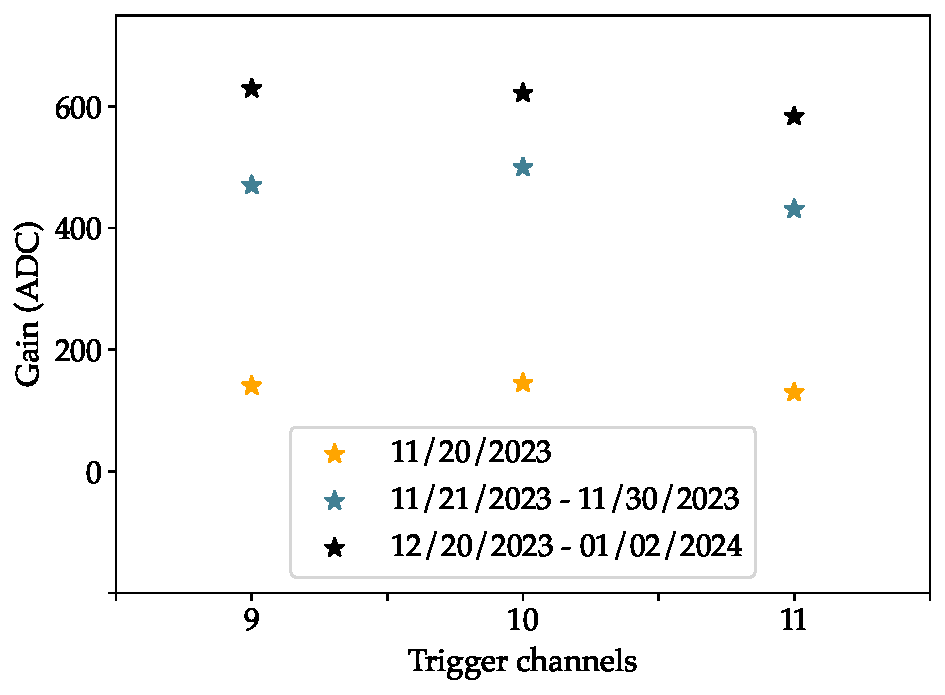
\includegraphics[width=11cm]{Gain_trigger_channels_BACoN_run2.pdf}
			\caption{Gain obtained for the trigger channels inside the BACoN detector for the different periods of data taken.}
			\label{fig:Gain_trigger_channels_BACoN_run2}
		\end{center}
	\end{figure}
	
	\subsection{First look at the peaks}
	
	For the data analysis is crucial to fully understand the shape of data and the peaks, since their amplitud (either height or integral) is related to the photons detected by each sensor. Figure \ref{fig:4event_example_channel8} shows different peaks zoomed in using a window of 1500 ns registered by the same channel. In most cases, an isolated single peak (that can correspond to few photoelectrons) is registered, but in many cases, before the peak goes down, more photons are detected, producing a second peak that is convoluted with the first one. Our analysis algorithm should take this into account and try to deconvolute both.
	
	\begin{figure}[!h]
		\begin{center}
			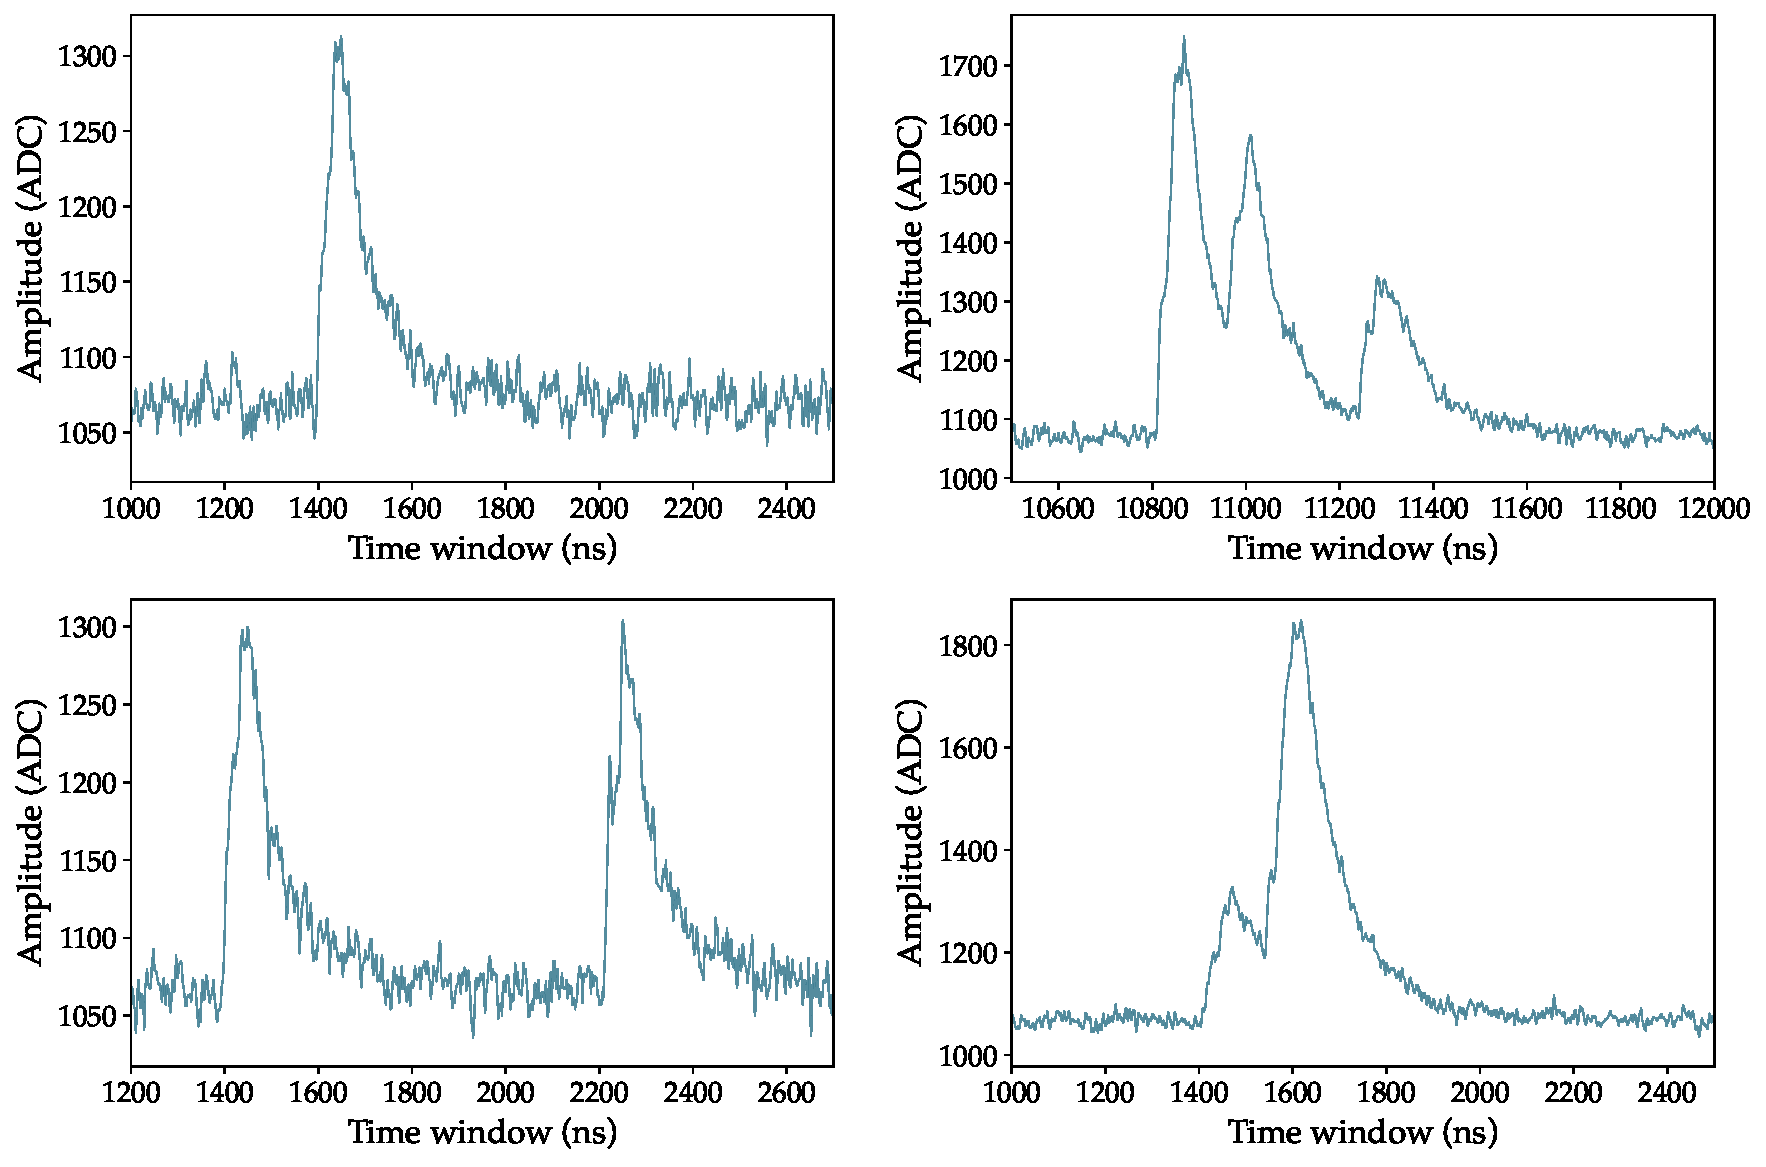
\includegraphics[width=16cm]{4event_example_channel8.pdf}
			\caption{Different kind of peaks selected for channel 8.}
			\label{fig:4event_example_channel8}
		\end{center}
	\end{figure}
	
	
	\subsection{Baseline subtraction}
	
	As mentioned in Section \ref{cal_dark_box}, it is necessary to subtract the baseline of each independent waveform to quantify the amount of light of the waveform either by using the height of the peaks or the integral. The baseline subtraction can be achieved by utilizing either the mean value or the mode of the entire waveform or by focusing on a specific range. In the BACoN data, we employ the range of the waveform just before the trigger region to minimize the impact of detected light on baseline computation, which could inflate its value. Furthermore, we opt for the mode as it has been determined to provide better accuracy in case a background event falls in the region before the trigger time.
	
	\begin{figure}[!h]
		\begin{center}
			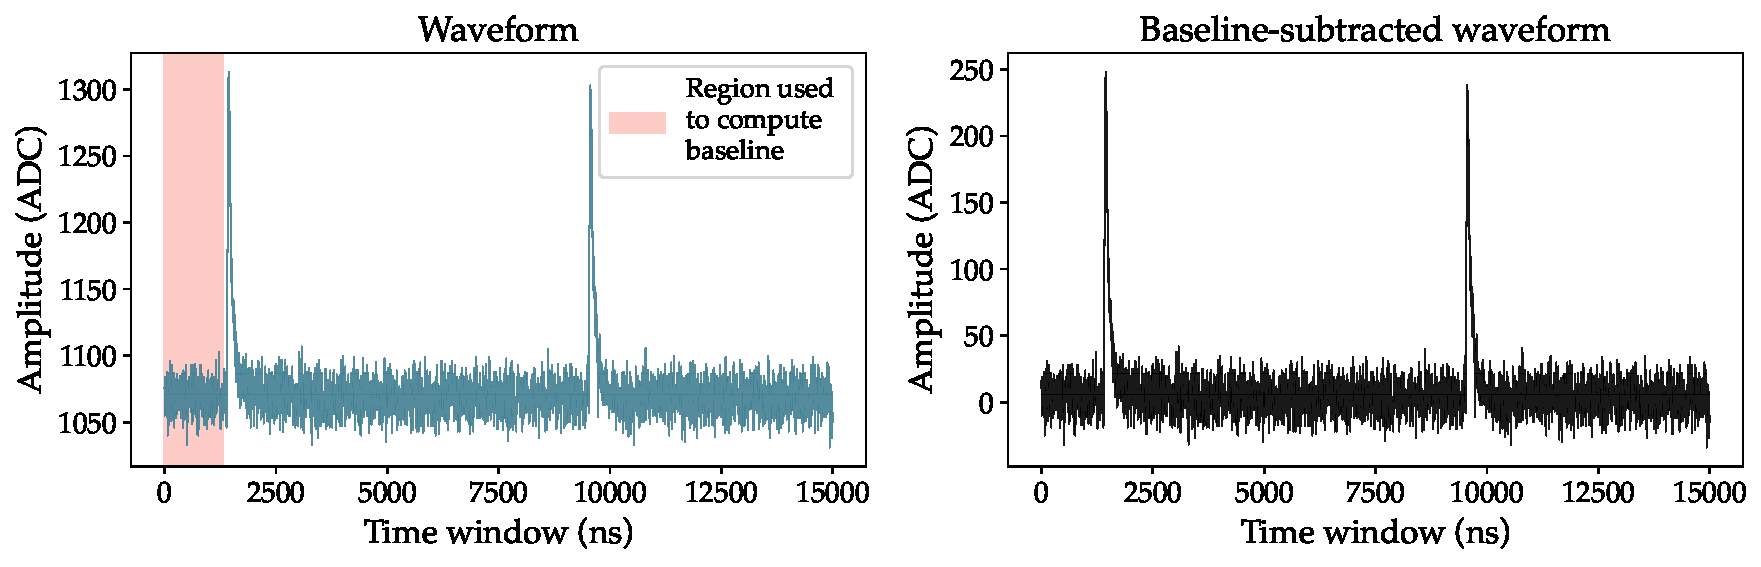
\includegraphics[width=16cm]{Baseline_subtraction_data.pdf}
			\caption{Left: original waveform showing in pink the time window used to compute the baseline using the mean or the mode. Right: Waveform after baseline subtraction.}
			\label{fig:Baseline_subtraction_data}
		\end{center}
	\end{figure}
	
	Figure \ref{fig:Baseline_subtraction_data} shows the waveform before (left) and after (right) baseline subtraction. In the plot on the left, the pink region indicates the area used to compute the baseline. Note that in the plot on the right, the baseline is centered at 0 ADC.
	
	
	\vspace{20pt}
	
	\subsection{Analysis methods}
	
	After baseline subtraction, there are two ways of analyzing waveforms, which can be complementary. The first one consists of summing all the waveforms for a channel (some cuts can be applied beforehand, such as cosmic cuts), and the second one consists of analyzing the hits (the peaks) and the times when the peaks occur.
	
	
	\subsubsection{Summing waveforms}
	
	This method is the simplest one in order to study the scintillation light model and extract the decay constants from the fit to understand the difference in the light yield and times after adding xenon. After summing the selected waveforms, the result must be normalized with the number of events summed and the gain extracted from the calibration procedure (Figure \ref{fig:summed_wfs_example}).
	
	\begin{figure}[!h]
		\begin{center}
			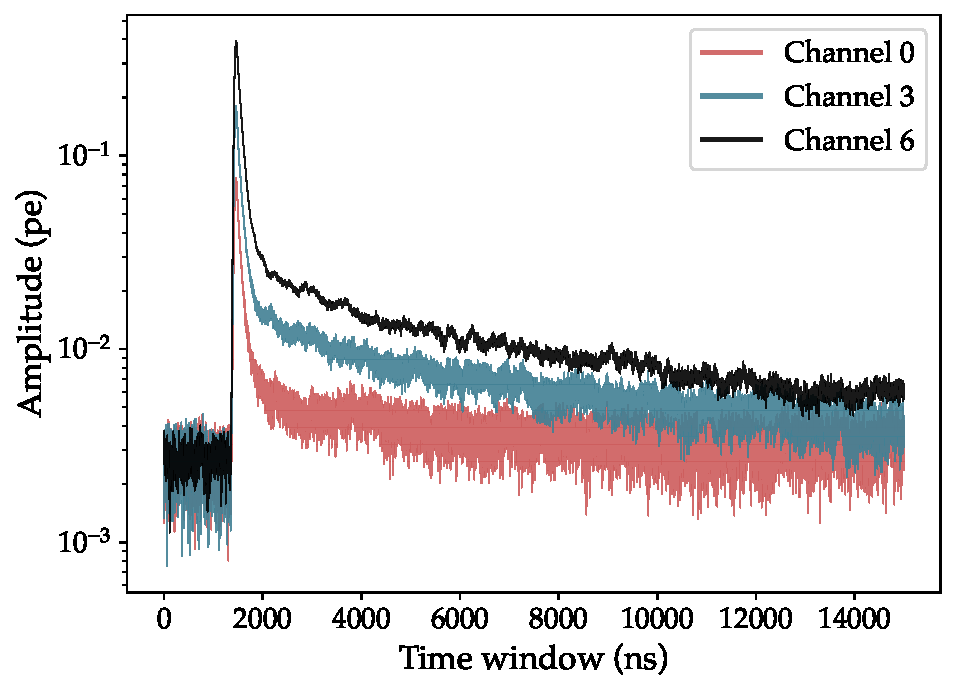
\includegraphics[width=11cm]{summed_wfs_example_norm_gain_and_evts.pdf}
			\caption{Average calibrated waveforms for channels 0, 3 and 6.}
			\label{fig:summed_wfs_example}
		\end{center}
	\end{figure}
	
	
	To reduce background events, we can remove waveforms that have peaks above a certain threshold before the trigger region. This is because the signal in the trigger region marks the start of the event. Therefore, the three trigger channels should record signals above 1 pe. If an event has a signal before the trigger time, it indicates that it does not come from the decay source but rather from the environment and should be rejected. Two examples of such waveforms are illustrated in Figure \ref{fig:Two_evts_with_signal_before_trigger_ch8}. The number of waveforms with a signal before the trigger time depends on the channel and the file, but ranges from 50 to 200 waveforms per data file.
	
	\begin{figure}[!h]
		\begin{center}
			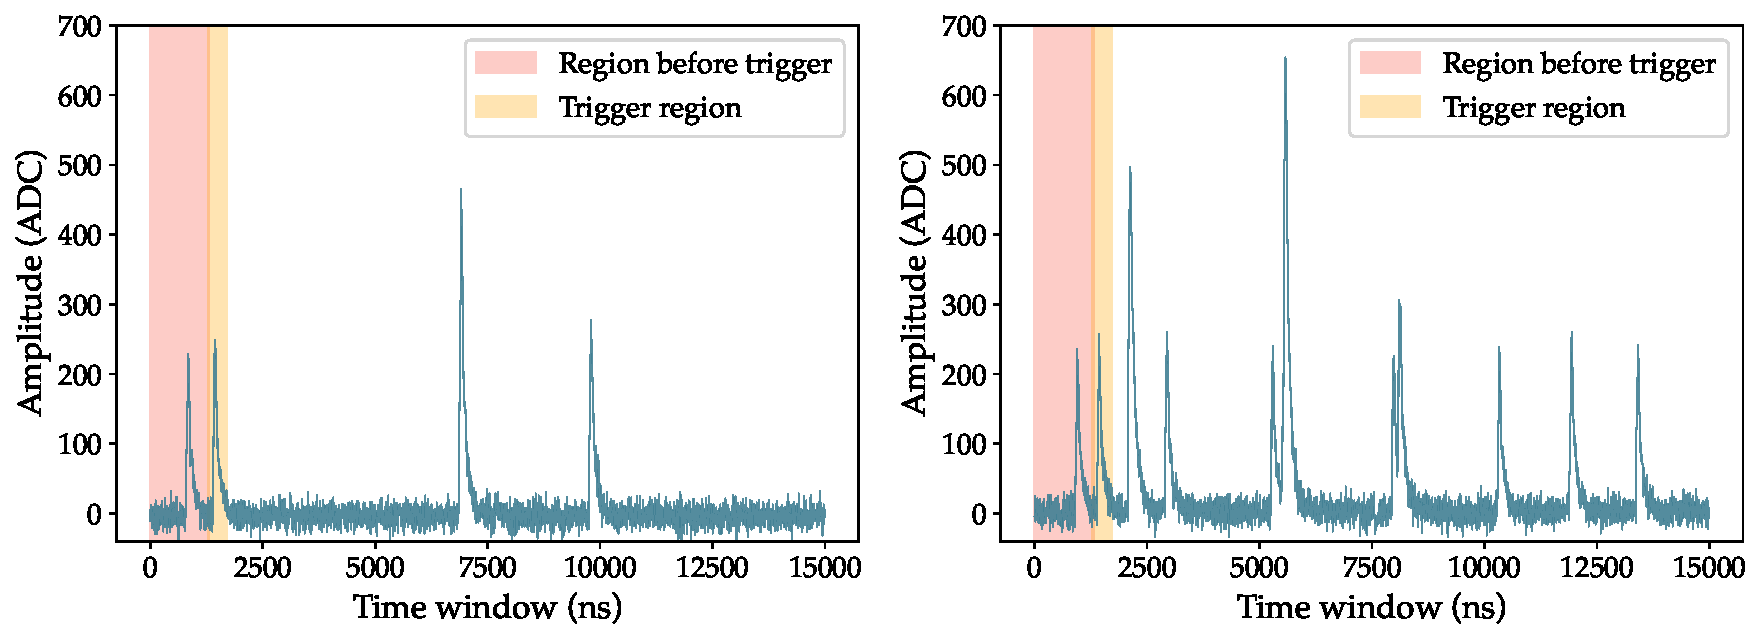
\includegraphics[width=16cm]{Two_evts_with_signal_before_trigger_ch8.pdf}
			\caption{Example of two background events (both present a peak before the trigger time).}
			\label{fig:Two_evts_with_signal_before_trigger_ch8}
		\end{center}
	\end{figure}
	
	\subsubsection{Analysis of hits}
	
	To identify valid hits in each channel waveform, the following steps are carried out:
	
	\subsubsection*{Smoothing waveforms using the Savitzky-Golay filter}
	
	First, it is necessary to apply a threshold to reject noise. However, noise counts could be mistaken for signal if they exceed the selected threshold. To mitigate this issue, we employ the Savitzky-Golay (SG) filter. This filter effectively removes noise from signals while preserving important features such as peaks and valleys. It is particularly useful when dealing with noisy data, enabling clearer analysis of the underlying signal.
	
	\begin{figure}[!h]
		\begin{center}
			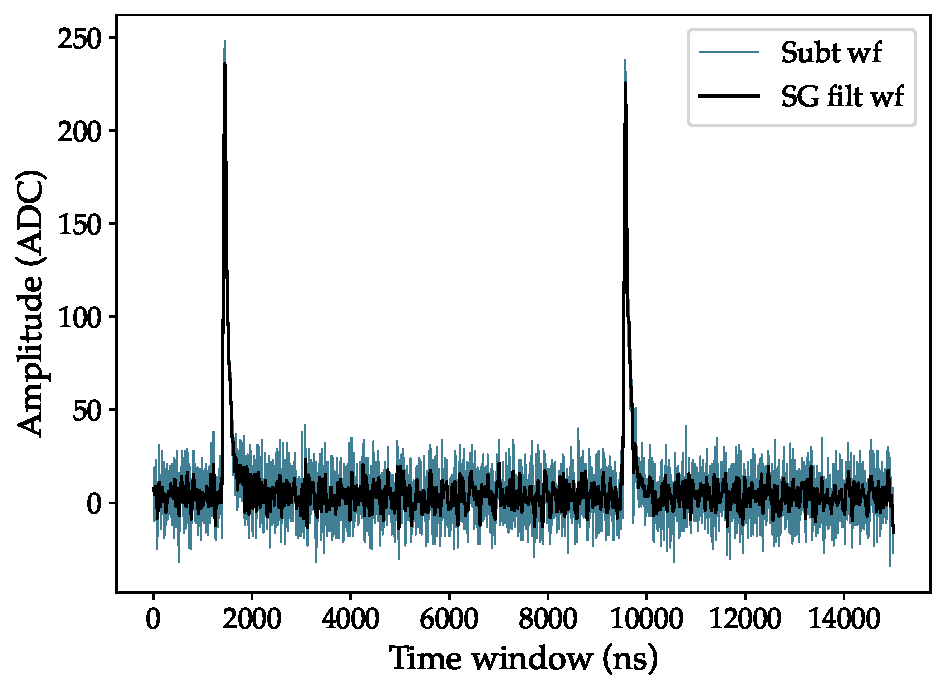
\includegraphics[width=11cm]{SG_waveform_wl30ns.pdf}
			\caption{Subtracted waveform (black) and waveform (salmon) after applying the Savitzky-Golay filter.}
			\label{fig:SG_waveform}
		\end{center}
	\end{figure}
	
	Figure \ref{fig:SG_waveform} shows a subtracted waveform and the result after filtering using the Savitzky-Golay (SG) filter. As depicted in Figure \ref{fig:SG_waveform_thr}, with this filter, we can ensure that no counts from the baseline exceed the desired threshold.
	
	\begin{figure}[!h]
		\begin{center}
			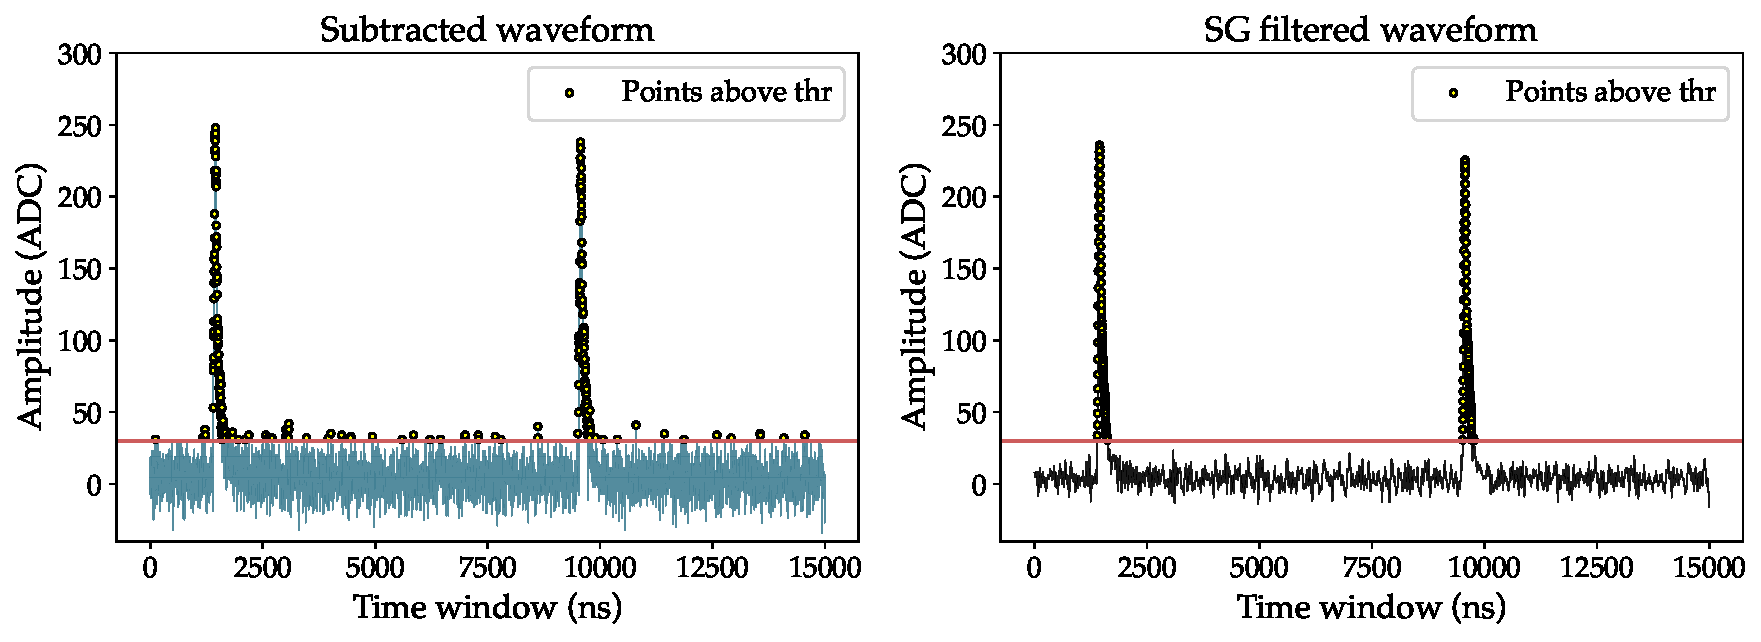
\includegraphics[width=16cm]{SG_waveform_wl30ns_thr_points.pdf}
			\caption{Left: subtracted waveform; right: subtracted and filtered waveform. The points above the chosen threshold (30 ADC, for example) have been plotted to illustrate that after filtering, no points from the baseline are present that could lead to a misinterpretation of the signal.}
			\label{fig:SG_waveform_thr}
		\end{center}
	\end{figure}
	
	One consideration when employing this method is that the heights of the peaks after filtering will be slightly reduced. Therefore, to address such variations, SiPM calibration should also be conducted using this method.
	
	\subsection*{Set a certain threshold and compute zero suppressed waveforms}
	
	An intermediate step between filtering and obtaining the peaks is to compute the zero-suppressed waveforms. In this process, all parts of the waveform below the chosen threshold, which removes the noise, will be converted into zeros (see Figure \ref{fig:ZS_waveform}). This makes it easier for the algorithm (which will be used and explained in the next step) to identify the different peaks.
	
	\begin{figure}[!h]
		\begin{center}
			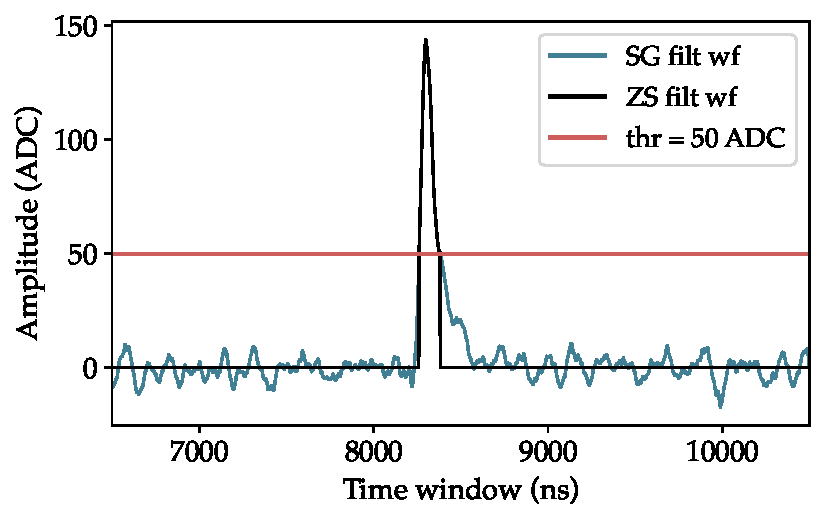
\includegraphics[width=11cm]{ZS_waveform.pdf}
			\caption{Peak of a selected waveform zoomed in. The blue curve corresponds to the filtered waveform while the black one is the zero suppressed waveform, where the values below 50 ADC have been set to zero.}
			\label{fig:ZS_waveform}
		\end{center}
	\end{figure}
	
	\subsection*{Search for peaks above the threshold}
	
	In order to get the peaks from our zero suppressed waveforms, we are using the python package \href{https://pypi.org/project/PeakUtils/}{\texttt{PeakUtils}}. As written in the documentation: "this package provides utilities related to the detection of peaks on 1D data. Includes functions to estimate baselines, finding the indexes of peaks in the data and performing Gaussian fitting or centroid computation to further increase the resolution of the peak detection". We should provide this algorithm the minimum distance between peaks and the absolute threshold in ADC. For the moment we are using 50 ADC both for the threshold the minimum distance between peaks.
	
	The outcome of the algorithm is the peak position in the waveform and using that we can extract the peak height, shown in Figure \ref{fig:ZS_peaks_waveform}.
	
	\begin{figure}[!h]
		\begin{center}
			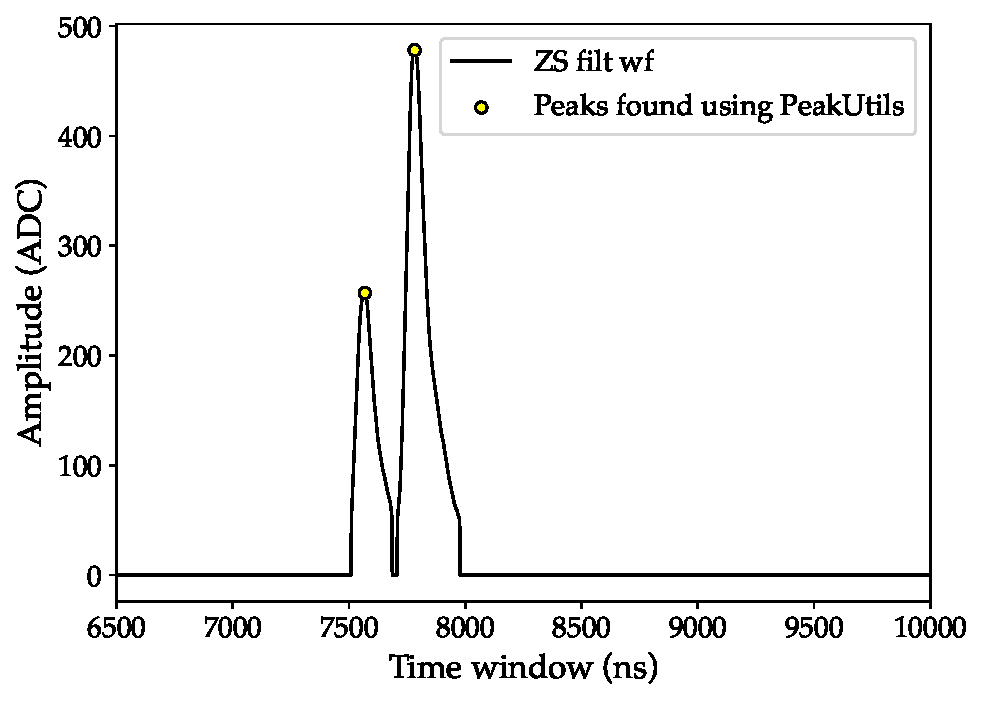
\includegraphics[width=11cm]{ZS_peaks_waveform.pdf}
			\caption{Example of the two peaks found by PeakUtils in a zero suppressed waveform.}
			\label{fig:ZS_peaks_waveform}
		\end{center}
	\end{figure}
	
	Using this method, we can get all the peaks from each channel and compute a hit map like the one shown in Figure \ref{fig:hit_map_example}. In the plot, defined horizontal lines can be observed. They are due to the invidividual photons registered by the SiPM.
	
	\begin{figure}[!h]
		\begin{center}
			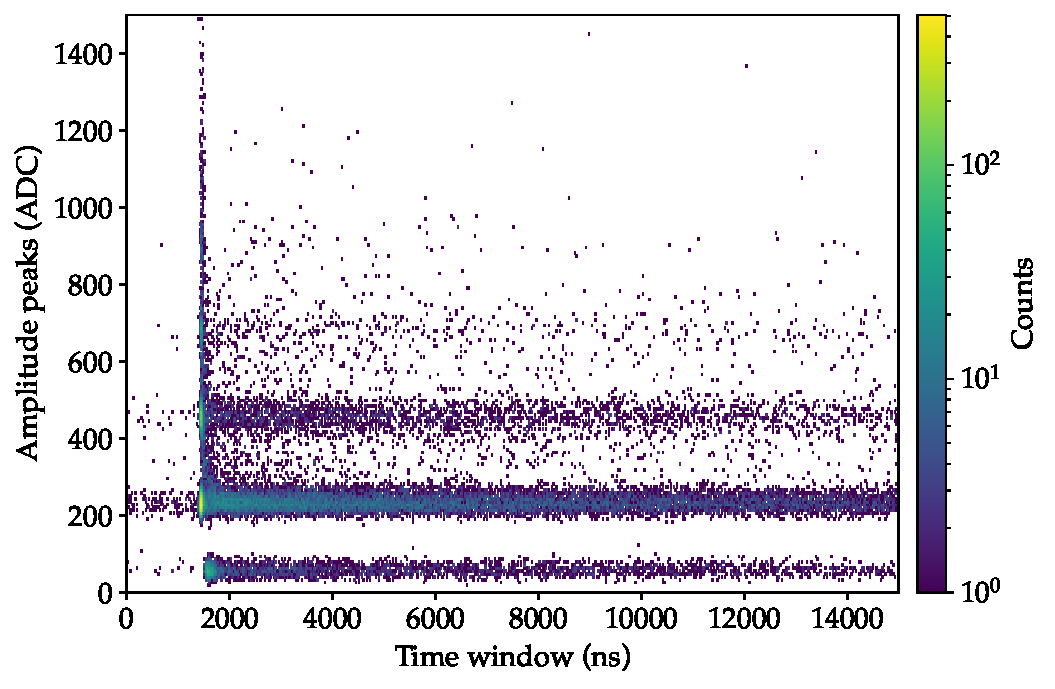
\includegraphics[width=12cm]{hit_map_example.pdf}
			\caption{Hit map for one channel. Each bin represents a peak with its timestamp (position in the waveform) and height (amplitude). Each horizontal line corresponds to a integer number of photoelectrons.}
			\label{fig:hit_map_example}
		\end{center}
	\end{figure}
	
	
	
	
	\subsection*{Additional ways to compute the hit map}
	
	In the previous method, we were taking the timestamp of the peak as the one corresponding to the maximum in the peak. However, another option is to take the time when the peak exceeds the threshold value. This way the effect of the rise time of each peak would be reduced (Figure \ref{fig:ZS_peak_waveform_thr}).
	
	\begin{figure}[!h]
		\begin{center}
			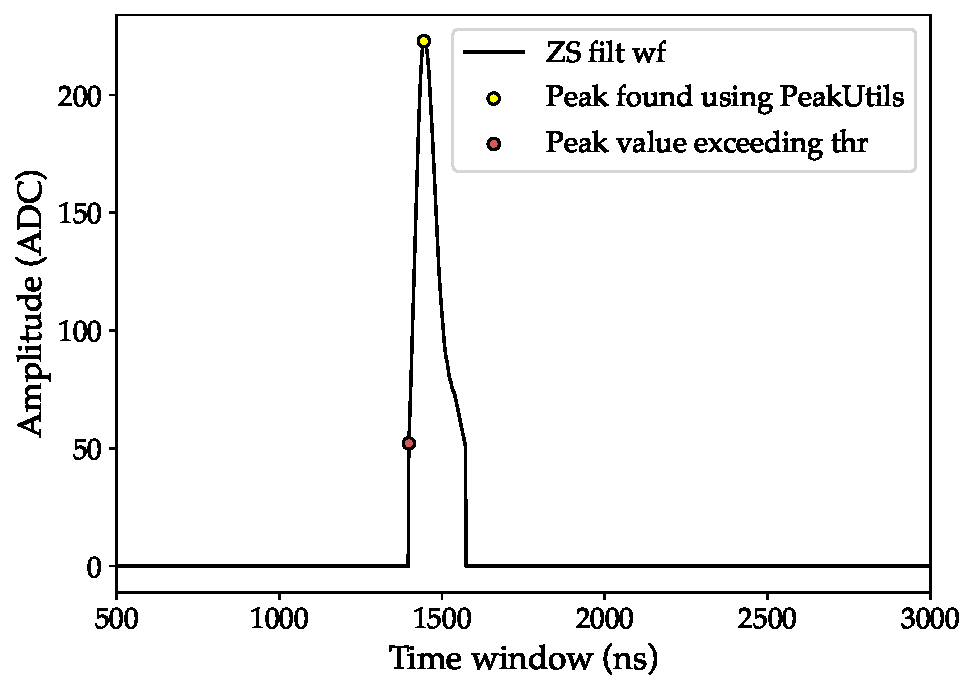
\includegraphics[width=11cm]{ZS_peak_waveform_thr.pdf}
			\caption{Example of a peak where the timestamp is taken from the maximum of the peak (yellow) or from the point where the threshold is exceeded (red).}
			\label{fig:ZS_peak_waveform_thr}
		\end{center}
	\end{figure}
	
	Another factor that we should take into account is the height of the peaks when two peaks overlap. If the second peak starts before the first peak reaches the baseline, the height of the second peak should start from the intersection with the first peak, as shown in Figure \ref{fig:ZS_peak_waveform_2nd_peak_minus_1st}.
	
	\begin{figure}[!h]
		\begin{center}
			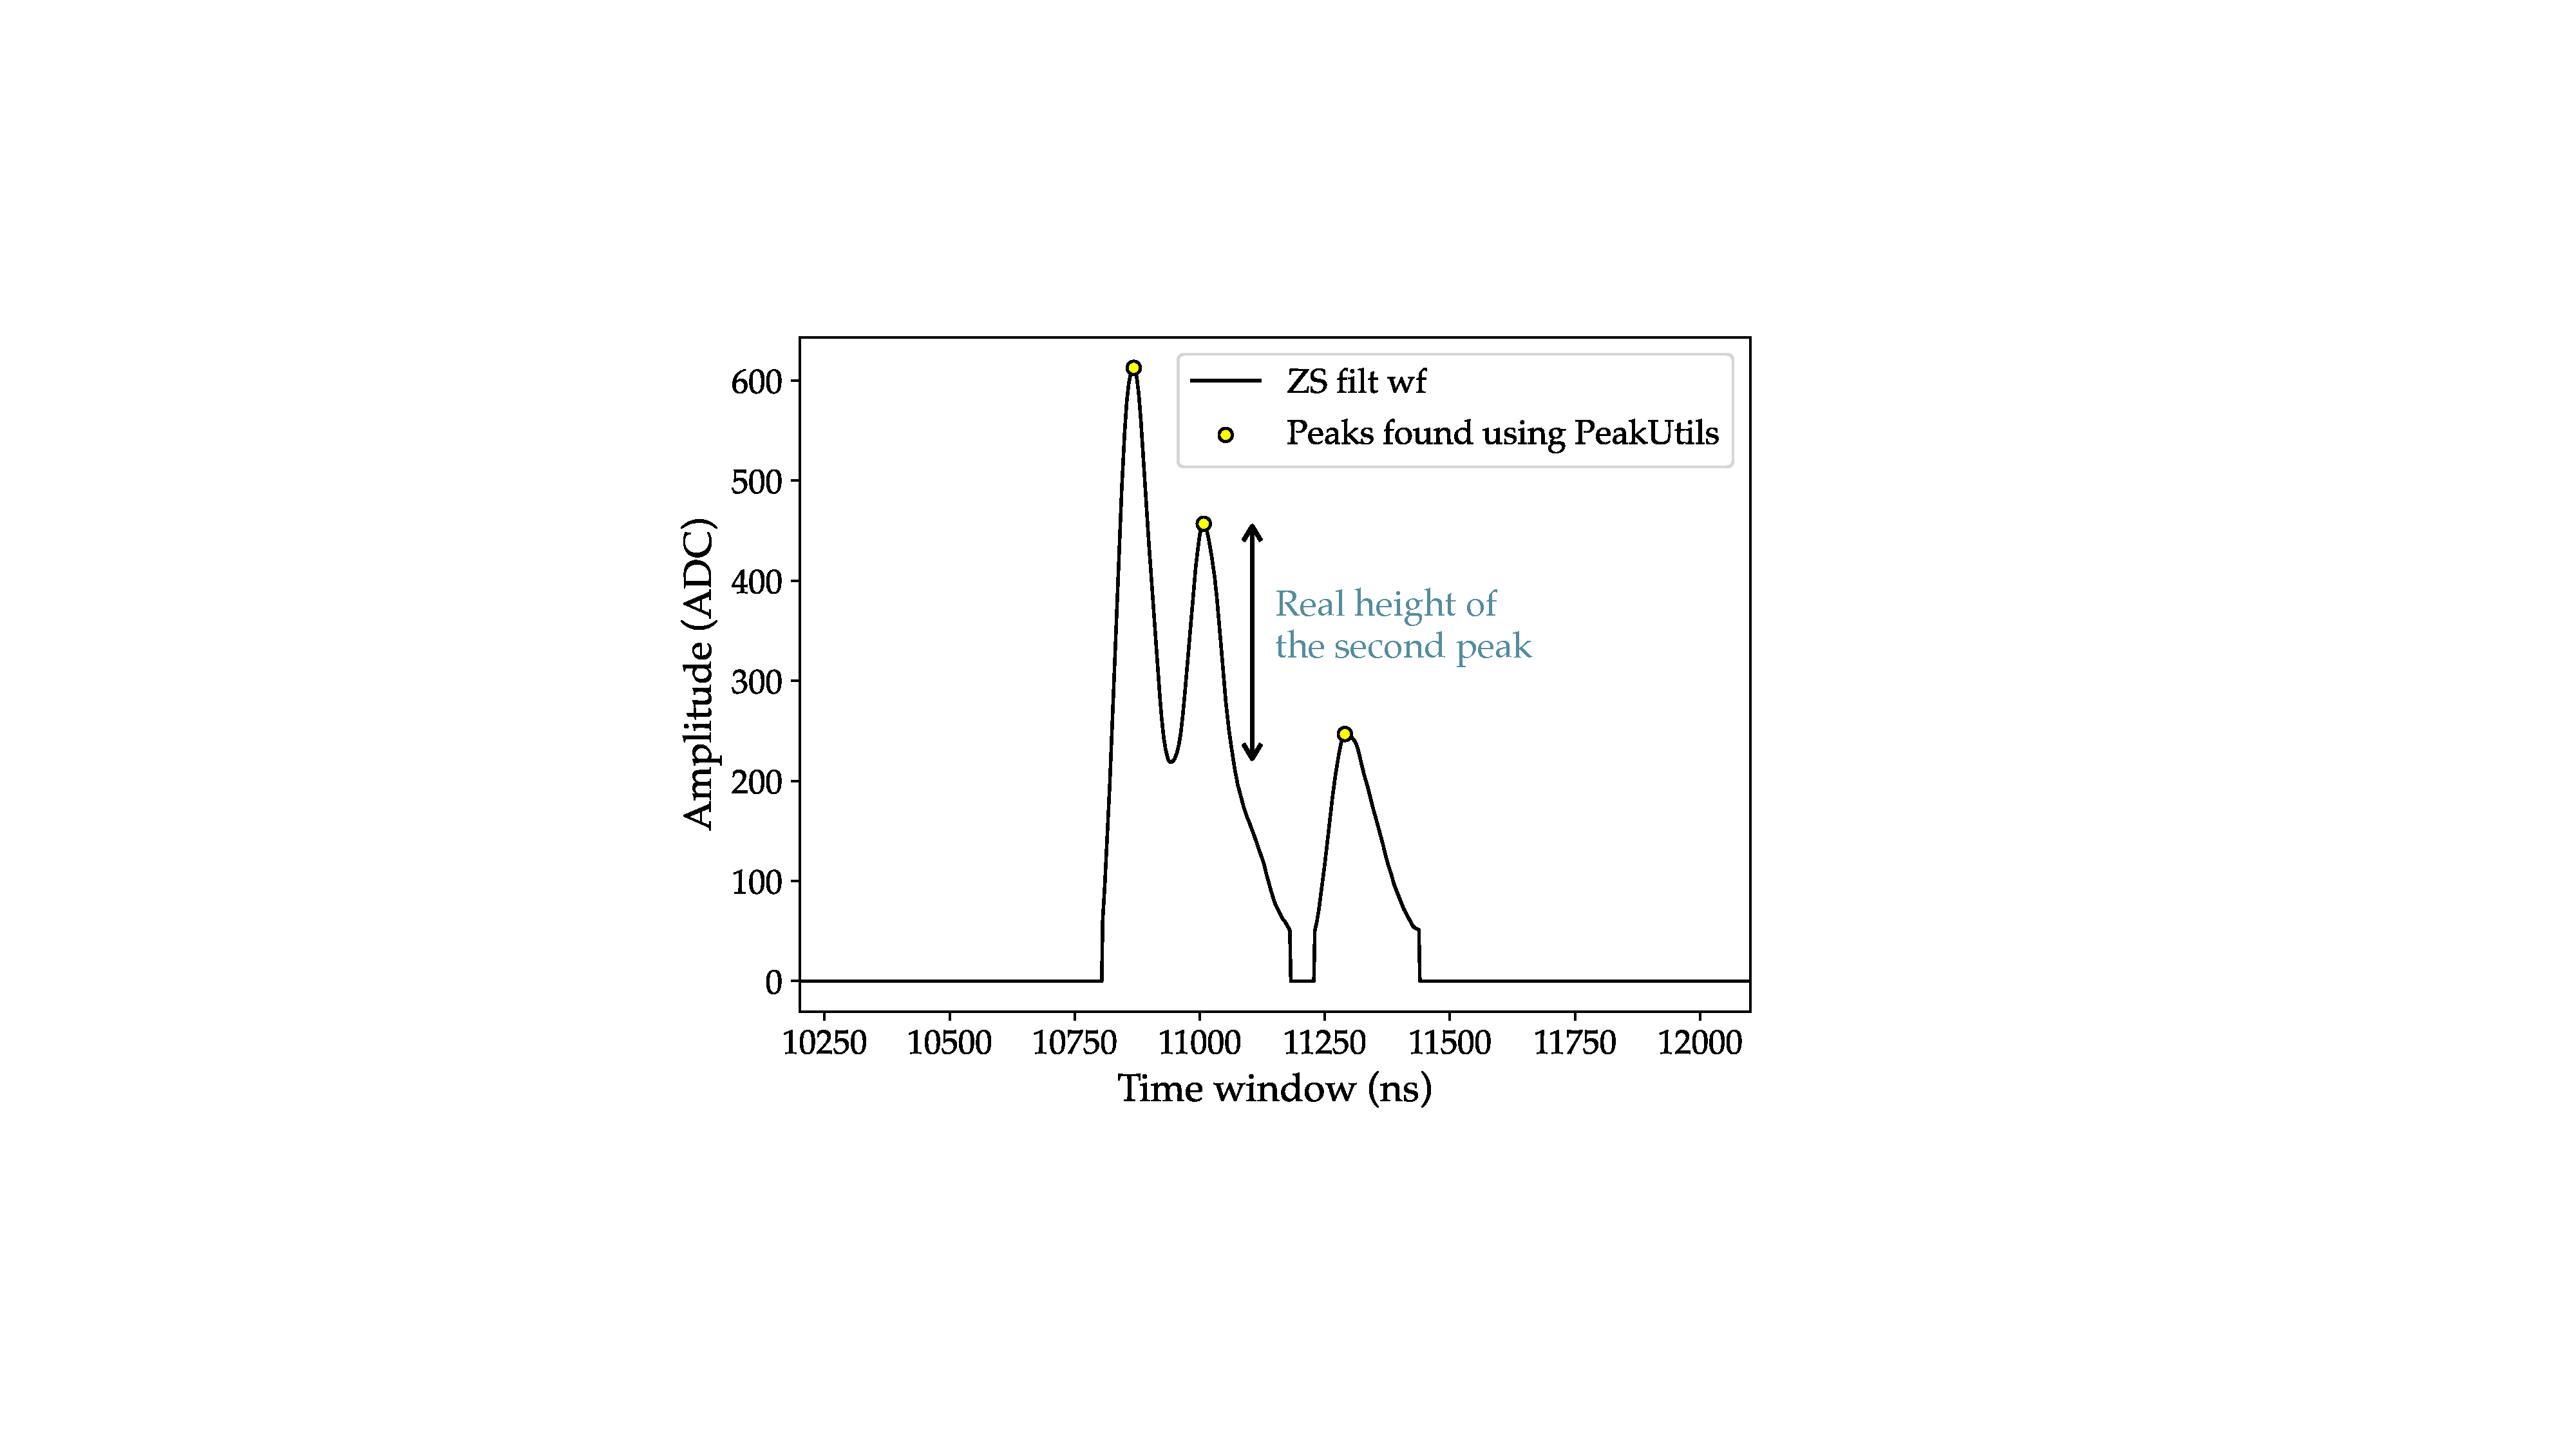
\includegraphics[width=11cm]{ZS_peak_waveform_2nd_peak_minus_1st_label.pdf}
			\caption{Example of two peaks overlapping. As it is written in the figure, the real height of the second peak corresponds to the difference between its height and the height of the intersection with the first peak.}
			\label{fig:ZS_peak_waveform_2nd_peak_minus_1st}
		\end{center}
	\end{figure}

	
	After combining the calibrated hits from all channels of a single file, the resulting hit map is depicted in Figure \ref{fig:hit_map_all_chs_spe} left. Subsequently, when the hits for each number of photoelectrons (represented by different colors up to 4 SPE) are aggregated into a histogram, Figure \ref{fig:hit_map_all_chs_spe} right is generated. It is observed that few number of photoelectrons are more common in the waveforms.
	
	\begin{figure}[!h]
		\centering
		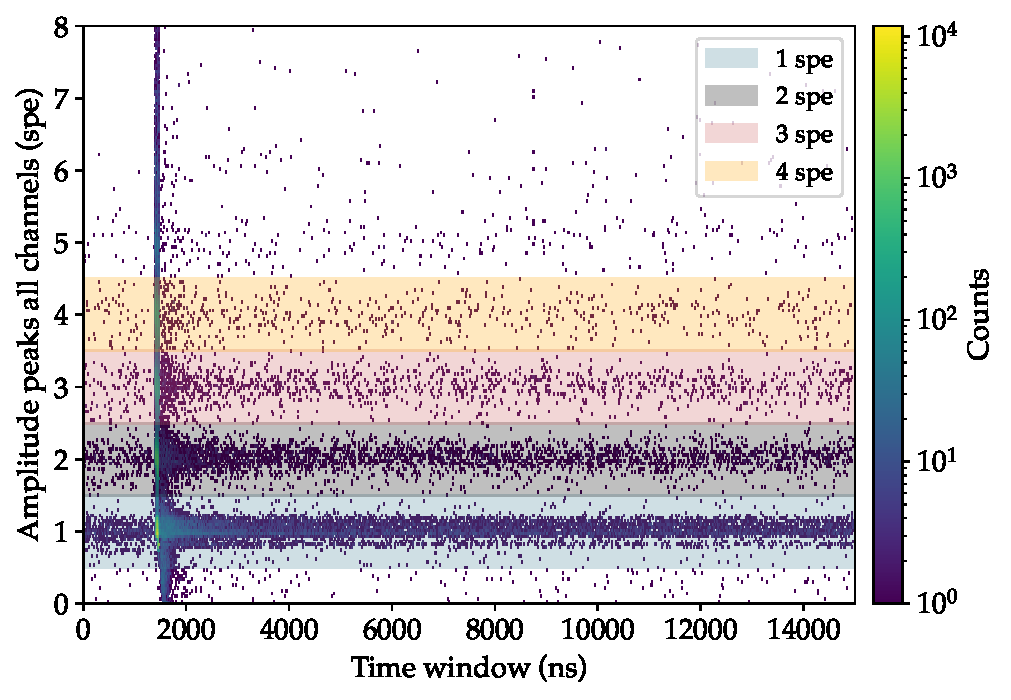
\includegraphics[width=7.9cm]{hit_map_all_chs_spe.pdf}
		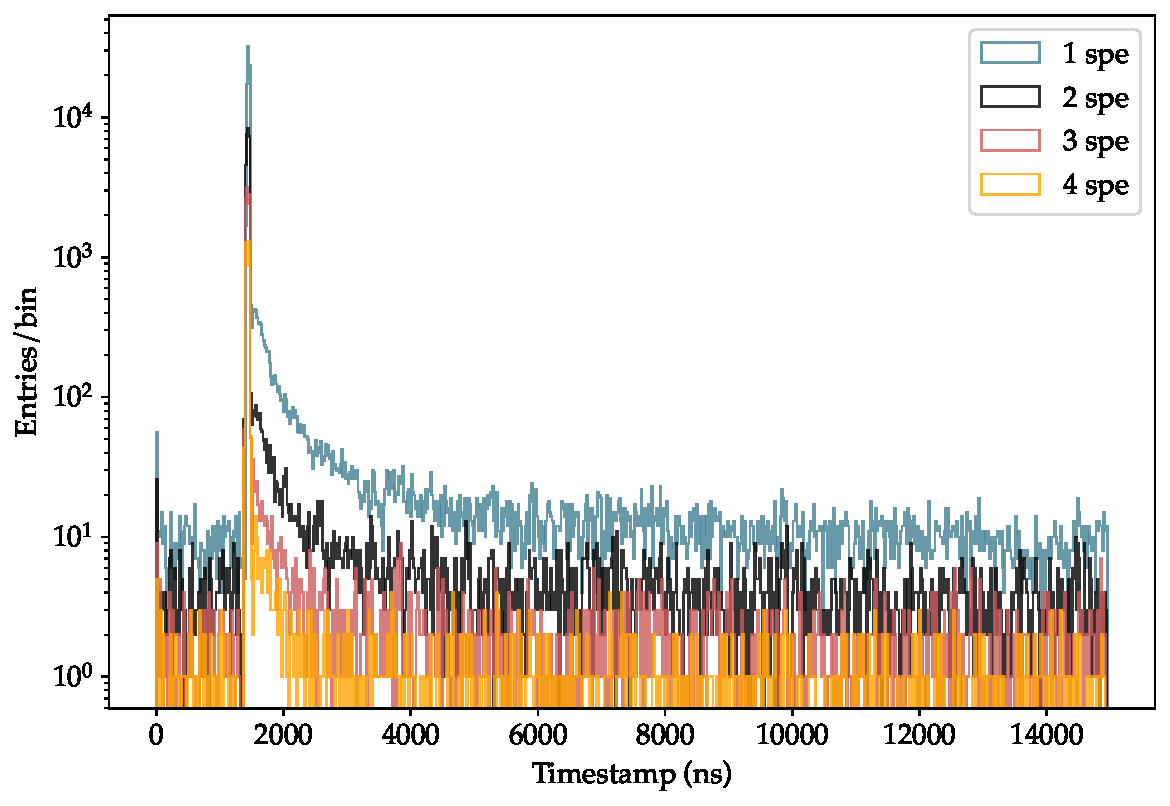
\includegraphics[width=7.9cm]{sum_hits_all_chs_spe.pdf}
		\caption{Left: calibrated hit map for all channels of a file with the colored bands corresponding to a different photon number. Right: histograms corresponding for each phoelectron number until 4 SPE.}
		\label{fig:hit_map_all_chs_spe}
	\end{figure}
	
	
	\subsection{Comparison between hit map and waveforms sum}
	
	Figure \ref{fig:hit_map_and_summed_wfs_norm} shows the comparison between the different analyses. The red line corresponds to the sum of the hits for each timestamp using the time of the maximum of each peak. The blue line has been computed also from the hit map but computing the time of the waveform when it crosses the threshold. Finally, the black line corresponds to the sum of all the waveforms in the selected file. All cases consider all the events with no signal before the trigger rate.
	
	\begin{figure}[!h]
		\begin{center}
			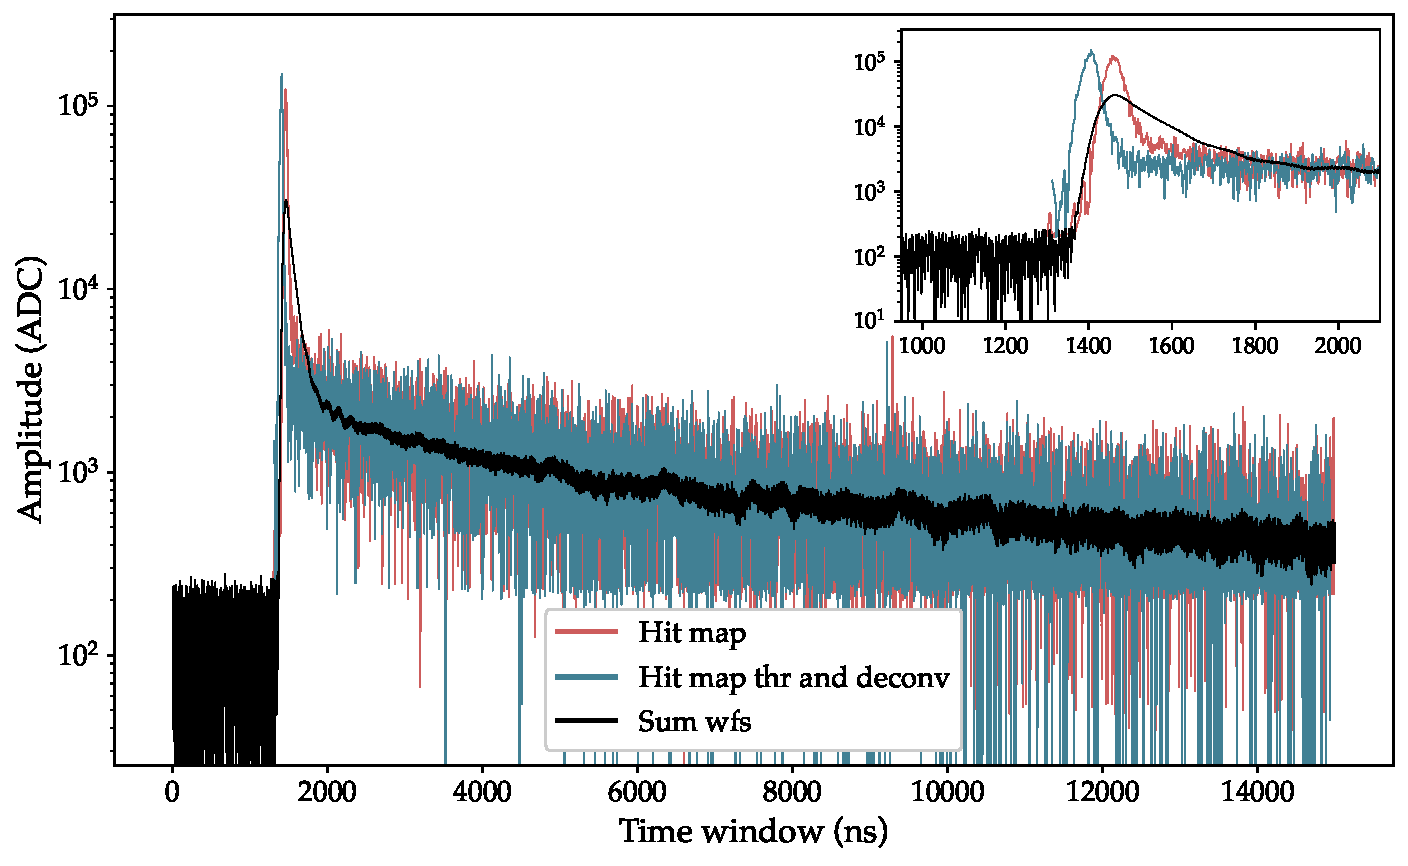
\includegraphics[width=15cm]{hit_map_and_summed_wfs_norm.pdf}
			\caption{Comparison between the analysis using the hit map with the time of the maximum of the peak (red) and using the time where the waveform exceeds the threshold and deconvolving the second peak from the first peak (blue) and the analysis using the sum of the waveforms (black), all three cases after removing events with peaks occurring before the trigger time. The sum of the waveforms has been normalized to achieve a similar order of magnitude as the other cases, enabling a comparison of the shapes of the three analyses. The plot on the upper right corner zooms in the peak region.}
			\label{fig:hit_map_and_summed_wfs_norm}
		\end{center}
	\end{figure}
	
	
	
	\section{Single photoelectron shape}
	
	Peak shape for the different number of photoelectrons.
	
	\begin{figure}[!h]
		\begin{center}
			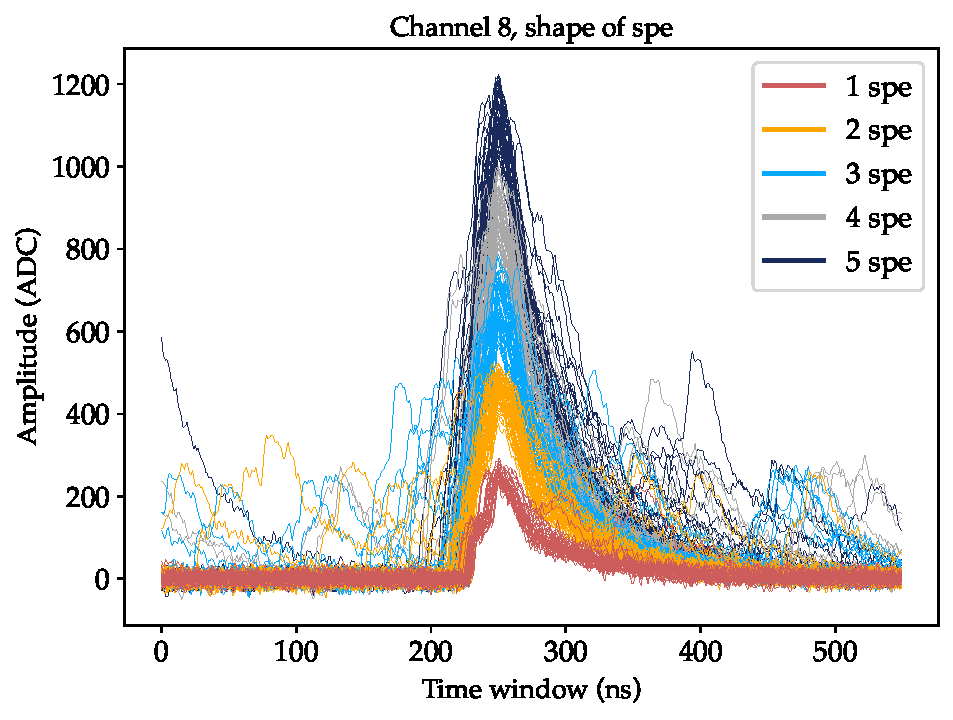
\includegraphics[width=11cm]{spe_shape.pdf}
			\caption{}
			\label{fig:spe_shape}
		\end{center}
	\end{figure}
	
	Fit of the 1 spe shape.
	
	\begin{figure}[!h]
		\centering
		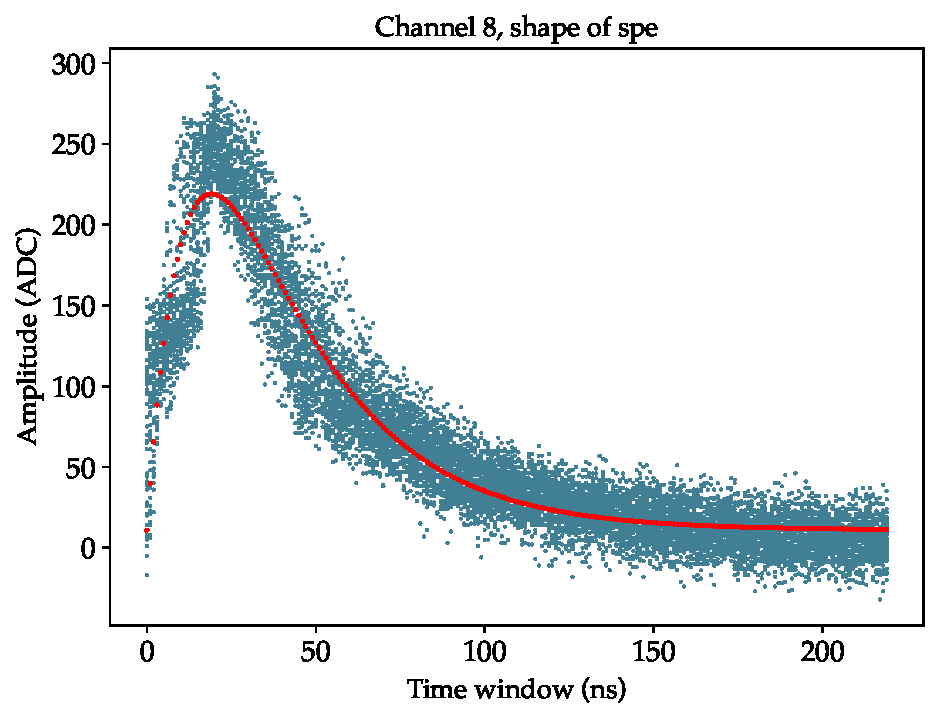
\includegraphics[width=7.9cm]{spe_shape_fit.pdf}
		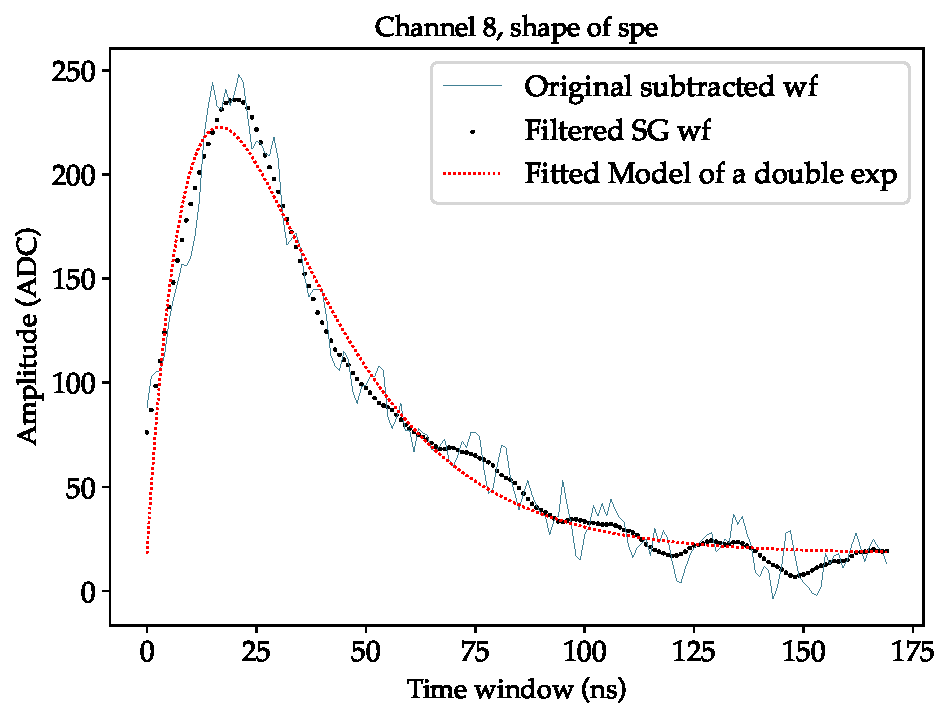
\includegraphics[width=7.9cm]{spe_shape_fit2.pdf}
		\caption{}
		\label{fig:spe_shape_fit}
	\end{figure}
	
	\section{Trigger time}
	
	We define the trigger time as the moment when the peak exceeds the threshold of 50 ADC in the trigger region of a waveform. Creating a histogram with the values for each channel results in the plots depicted in Figure \ref{fig:trigger_time}. On the left, the trigger time for the trigger SiPMs is displayed, while the plot on the right illustrates the same parameter for the regular SiPMs. In both cases, the peaks are centered around 710 ns, but the FWHM is narrower in the trigger SiPMs (clode to 40 ns, corresponding to the trigger window). This result was expected, as the trigger SiPMs are closer to the source.
	
	\begin{figure}[!h]
		\centering
		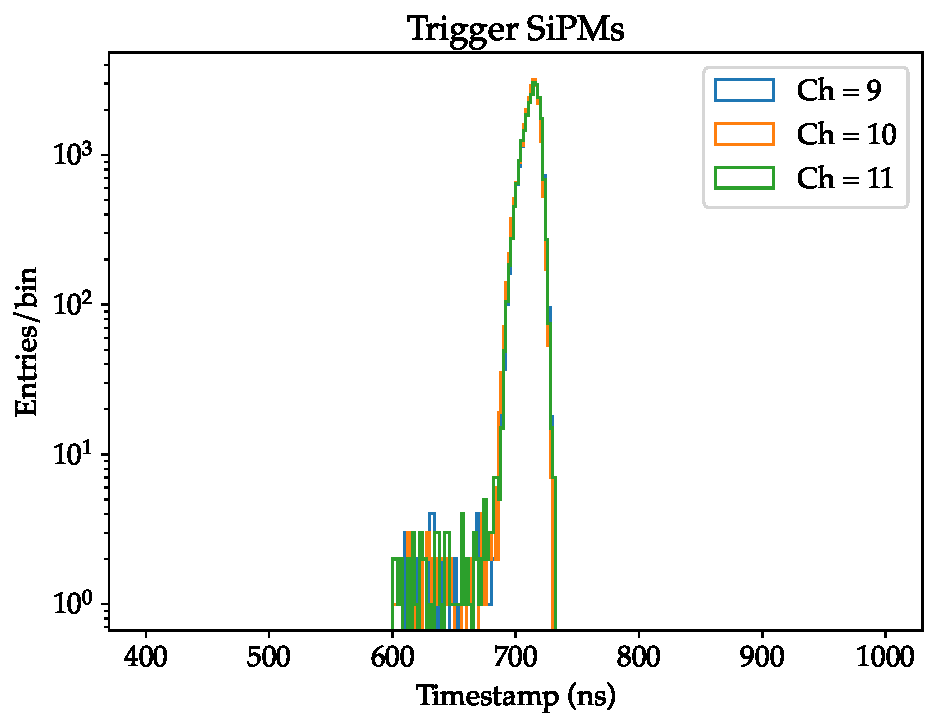
\includegraphics[width=7.9cm]{trigger_time_trigger_chs.pdf}
		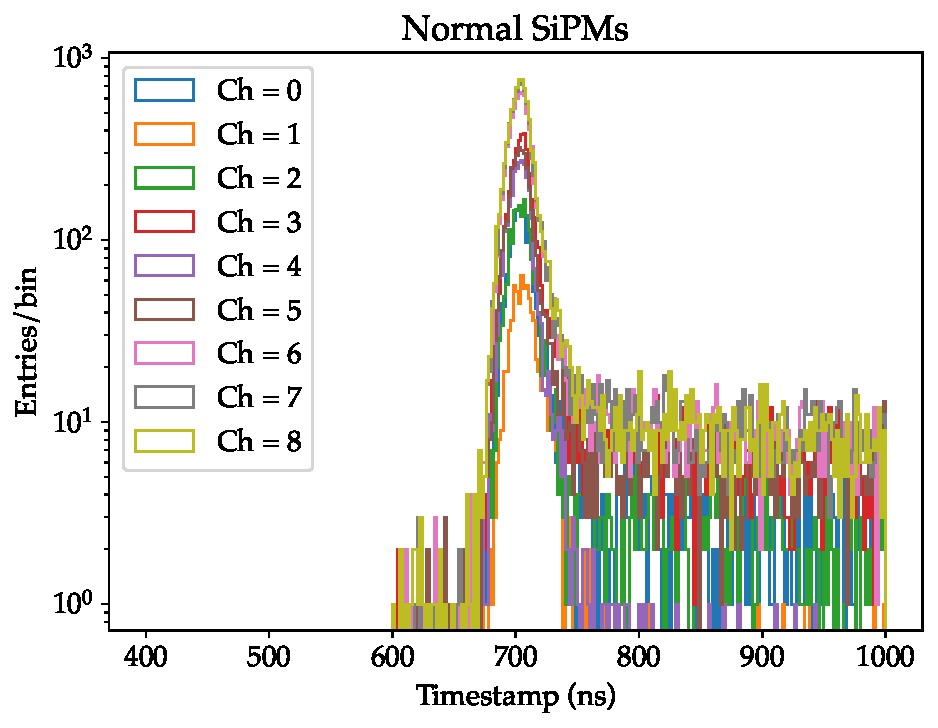
\includegraphics[width=7.9cm]{trigger_time_normal_chs.pdf}
		\caption{Trigger time for the trigger SiPMs (left) and for the regular SiPMs (right).}
		\label{fig:trigger_time}
	\end{figure}

	
	Plot \ref{fig:trigger_time_fit_trigger_and_regular} depicts a fit for the trigger time combined for the source SiPMs (left) and the regular SiPMs (right). The histogram shape of the trigger SiPMs is non-gaussian, whereas it appears more gaussian for the regular SiPMs. As mentioned, the width of the distribution is narrower for the source SiPMs.
	
	\begin{figure}[!h]
		\begin{center}
			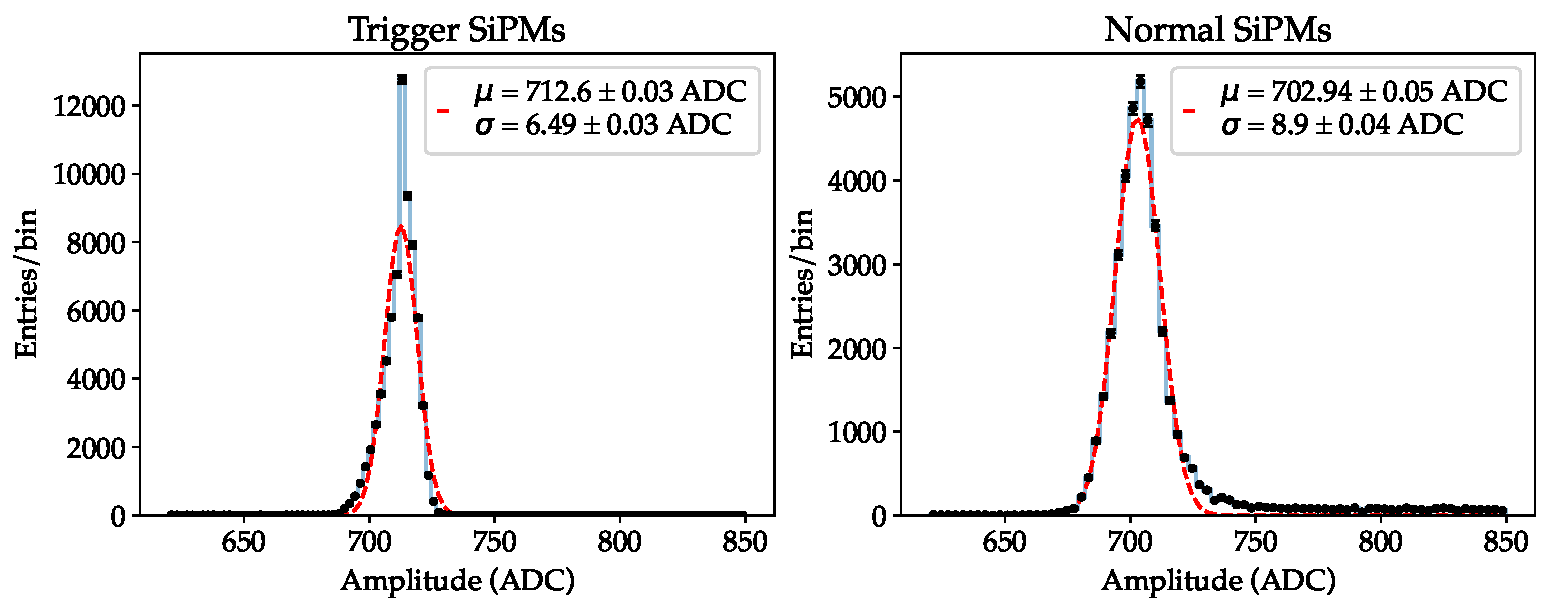
\includegraphics[width=16cm]{trigger_time_fit_trigger_and_regular.pdf}
			\caption{Fit of the trigger time combined for the trigger SiPMs (left) and the normal SiPMs (right).}
			\label{fig:trigger_time_fit_trigger_and_regular}
		\end{center}
	\end{figure}
	
	
	\section{Rise time}
	
	We are computing the rise time of the peaks as the difference between the maximum of the peak and the point that surpass the selected threshold.
	
	\begin{figure}[!h]
		\begin{center}
			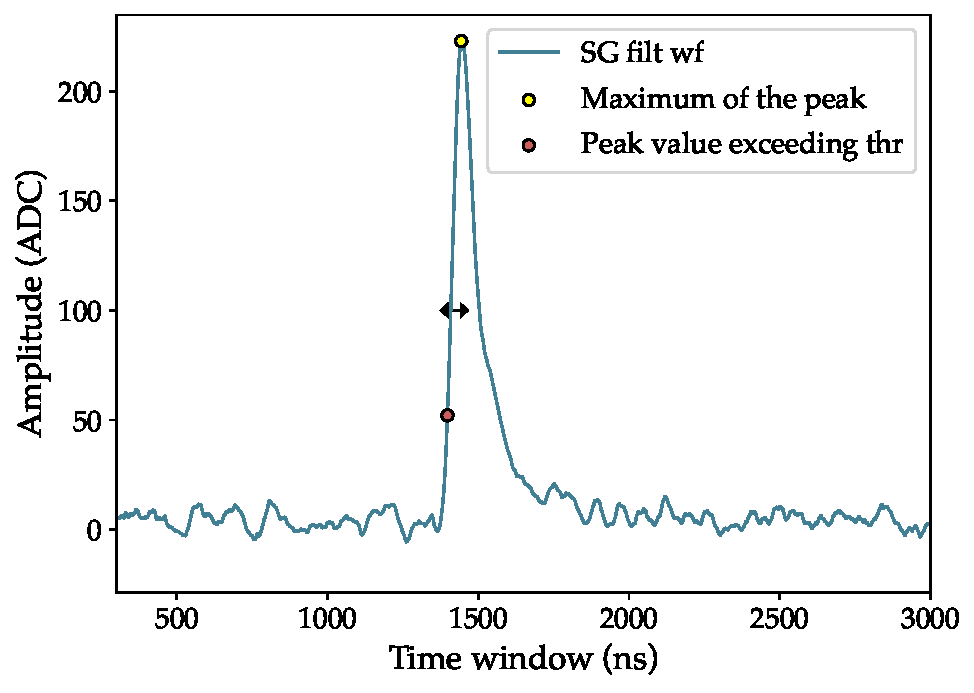
\includegraphics[width=10cm]{Rise_time_illustration.pdf}
			\caption{Waveform with the maximum in yellow and the point where the threshold of 50 ADC is exceeded in red. From the difference of the two times, the rise time is computed.}
			\label{fig:Rise_time_illustration}
		\end{center}
	\end{figure}
	
	Figure \ref{fig:rise_time} shows the rise time vs amplitude in number of photoelectrons for all SiPMs. As expected, the rise time of a peak increases with the number of photoelectrons.
	
	\begin{figure}[!h]
		\begin{center}
			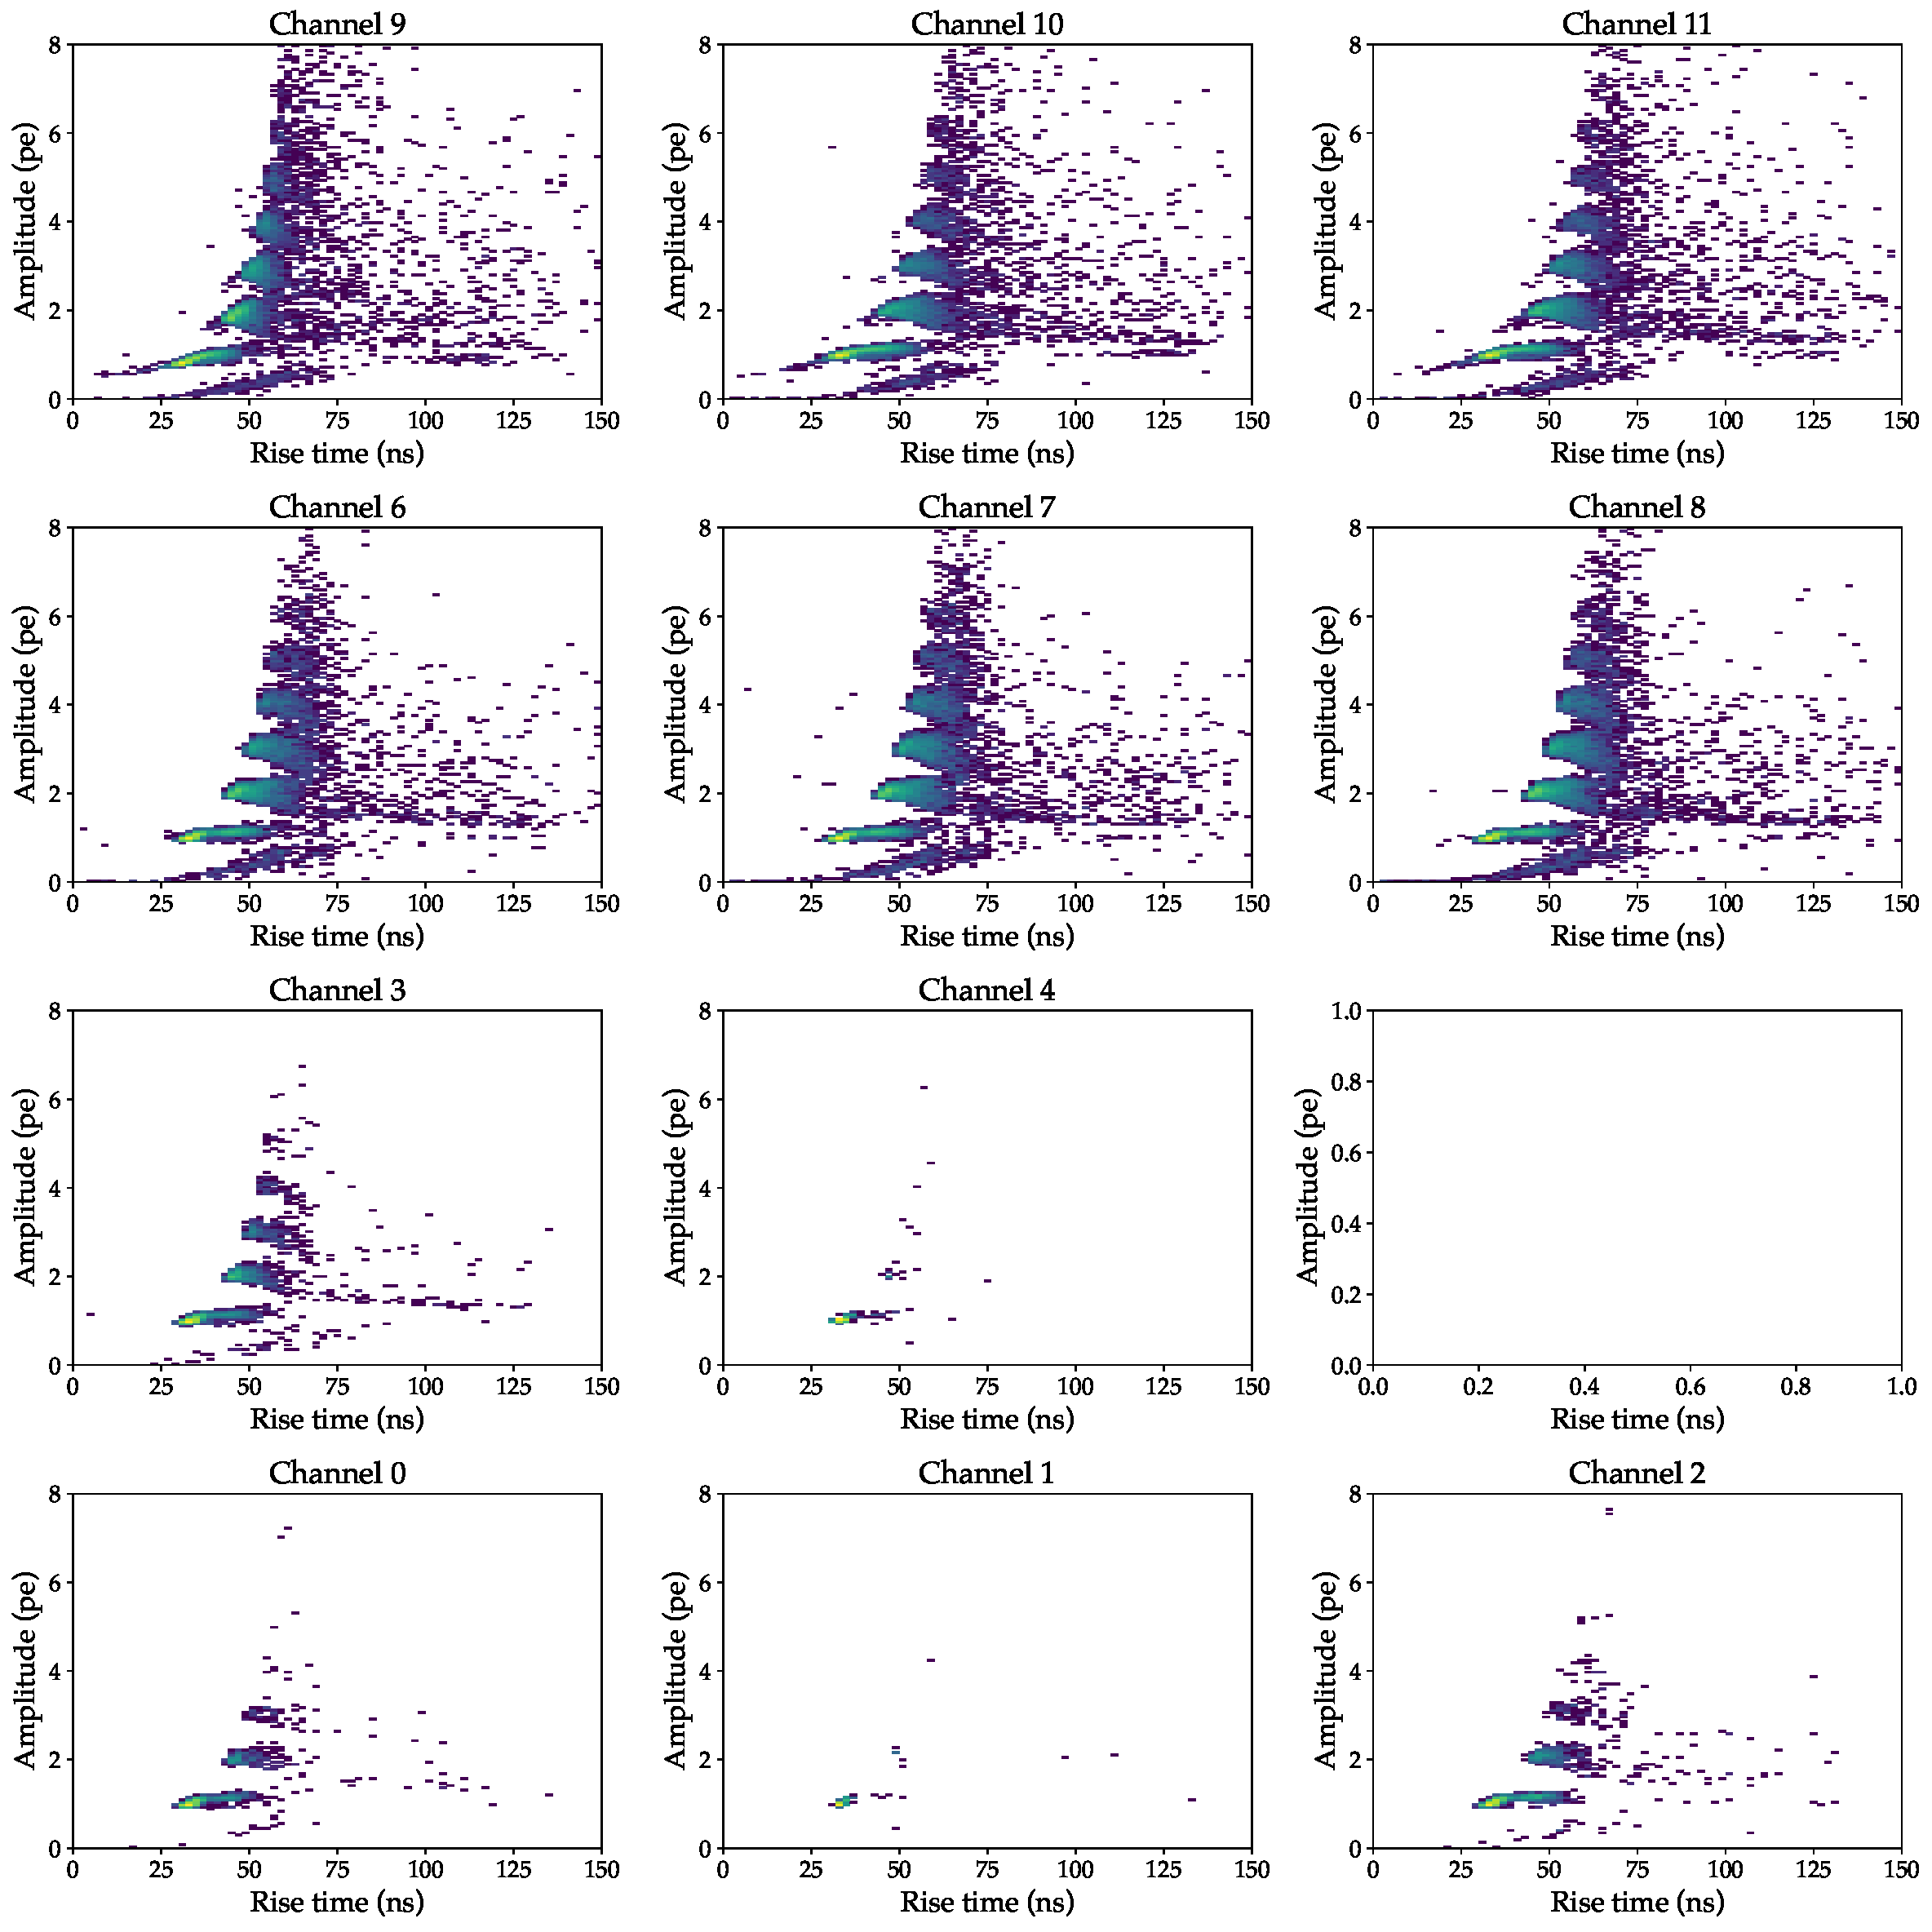
\includegraphics[width=16cm]{rise_time.pdf}
			\caption{Rise time versus number of photoelectrons for each channel for a Dec 28th run (first file). Channels 9, 10 and 11 are the trigger SiPMs, close to the source. Channel 5 was not working correctly.}
			\label{fig:rise_time}
		\end{center}
	\end{figure}
	
	\section{Energy spectrum}
	
	The energy spectrum obtained with our setup can be computed using the amount of light detected by the three trigger SiPMs per event. Various scenarios are illustrated in Figure \ref{fig:Spectrum_trigger_SiPMs_all_runs_all_cases}: the sum of the peaks in the entire window versus the trigger window, and all events versus only centered events. Centered events are selected by summing only the charges of each channel within a difference of 2 pe with the other 2 channels. This way, we can ensure that the event occurred at a similar distance from all sensors, that is, at their center.
	
	\begin{figure}[!h]
		\begin{center}
			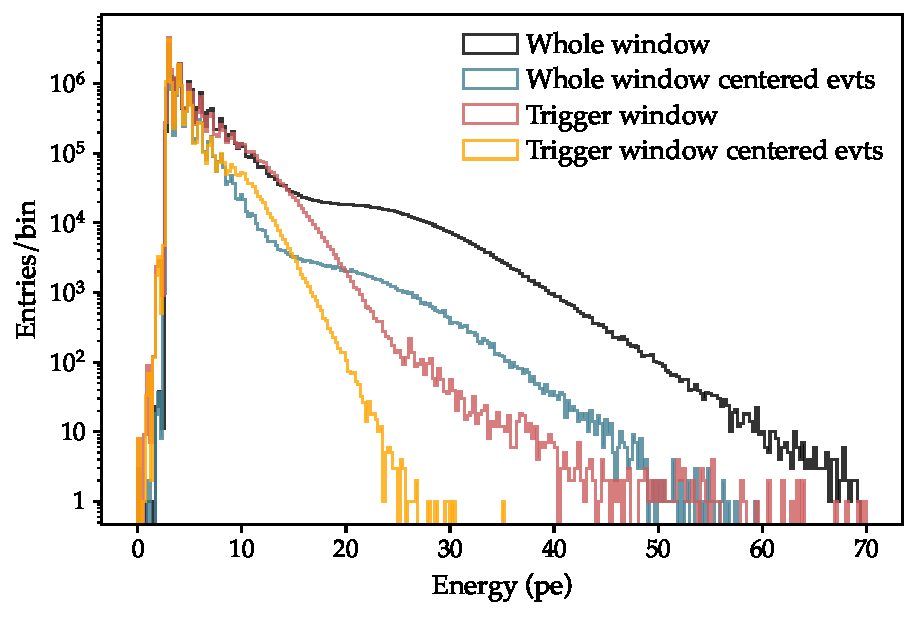
\includegraphics[width=10cm]{Spectrum_trigger_SiPMs_all_runs_all_cases_leg_style.pdf}
			\caption{Summed energy of the three trigger SiPMs for 4 different cases: taking the whole window of the event, taking only the trigger window, and the two same cases but selecting those events with $\pm$2 pe difference between the three channels.}
			\label{fig:Spectrum_trigger_SiPMs_all_runs_all_cases}
		\end{center}
	\end{figure}
	
	In Figure \ref{fig:Spectrum_trigger_SiPMs_all_runs_all_cases}, individual photoelectrons (starting at 3, since the sum is represented) are observable on the left. Near energy levels corresponding to several photoelectrons, a subtle bump is noticeable in all cases. This bump is likely attributed to the alpha particles emitted by the source. Unlike the LLAMA detector, which exhibits a distinct peak resulting from gamma rays at around 40 photoelectrons and no discernible peak for alphas, our setup displays a minor bump indicative of alphas, but an indistinguishable gamma peak. Several disparities exist between the two detectors: LLAMA's underground location results in fewer background interferences. Additionally, they employ a higher threshold in the electronics of their trigger SiPMs, and their source is sealed, precluding alpha particle detection. Furthermore, their SiPMs lack collimation, resulting in a higher acceptance, approximately 2 orders of magnitude more than in BACoN. Therefore, it is reasonable that in our setup, the alpha peak appears at a lower energy region0.

\end{document}